\documentclass[a4paper, 12pt]{article}

\usepackage{graphicx}
\usepackage[font=small, labelfont=bf, labelsep=colon]{caption}
\usepackage{amsmath, amssymb}
\usepackage{float}
\usepackage{textcomp}
\usepackage{siunitx}
\usepackage[dvipsnames]{xcolor}
\usepackage{titling} % To allow to use \matitle more than once
\usepackage{ctable}
\usepackage{multirow}
\usepackage[flushmargin, bottom]{footmisc} 
\usepackage{hyperref}

\hypersetup{
colorlinks = true,
linkcolor = {blue!80!black}
}

\graphicspath{{../../Pictures/}}

%%%%%%%%%%%%%%%%%%%%%%%%%%%%%%%%%%%%%%%%%%%%%%%%%%%%%%%
% Layout parameters 
\setlength{\parindent}{0em}
\setlength{\parskip}{2ex}
\linespread{1.2}

\renewcommand{\floatpagefraction}{.99} % Minimum fraction of floats, in a page that has only floats. Only figures taking up more than that will get their own page. Default 0.5
\renewcommand{\topfraction}{0.99}  % Maximum fraction of page for floats at top. I.e.: floats taking up more than this will have no text below. Default: 0.7.
\renewcommand{\textfraction}{0.01} % Minimum fraction of page that must have text (otherwise, the page will only have float). Default: 0.2 

\addtolength{\textwidth}{2cm}
\addtolength{\hoffset}{-1cm}
\setlength{\topmargin}{-1cm}
\addtolength{\textheight}{1cm}

\setlength{\skip\footins}{6mm} % space between end of text and horizontal line of footnote
\setlength{\footnotesep}{5mm} % space between footnote line and first entry, and between consecutive entries of footnote



%%%%%%%%%%%%%%%%%%%%%%%%%%%%%%%%%%%%%%%%%%%%%%%%%%

%%%%%%%%%%%%%%%%%%%%%%%%
%%%%% NEW COMMANDS
%%%%%%%%%%%%%%%%%%%%%%%%

% Text commands
\newcommand{\spc}{1ex}
\newcommand{\eg}{\textit{e.g.}}
\newcommand{\ie}{\textit{i.e.}}

% Maths Commands
\newcommand{\R}{\mathbb{R}}
\newcommand{\bd}[1]{\boldsymbol{#1}}
\newcommand{\x}{\bd x}
\newcommand{\A}{{_{[A]}}}
\newcommand{\xA}{\bd{x^\A}}
\newcommand{\eps}{\varepsilon}
\newcommand{\Nr}{N_\text{regr}}
\newcommand{\E}{\mathbb{E}}
\newcommand{\Var}{\text{Var}}

\newcommand{\D}{\mathcal{D}}


\newcommand{\ya}{y^{(\alpha)}}
\newcommand{\yb}{y^{(\beta)}}
\newcommand{\ta}{\bd{\widetilde \alpha}}
\newcommand{\tb}{\bd{\widetilde \beta}}



%%%%%%%%%%%%%%%%%%%%%%%%%%%%%%%%%%%%%%%%%%%%%%%%%%%%%

\title{First-Wave Emulators}

\author{}
\date{}

\begin{document}

\maketitle

\thispagestyle{empty}

\tableofcontents
\newpage

\setcounter{page}{1} 

\maketitle
\vspace{-9ex}

This document relates to the project with Mohammad Royapoor on the modeling of a building's energy consumption. I first recall what the setting and aim are, then detail the choices I have made to construct a first wave of emulators, and finally explore the history matching under some scenarios.


\section{The Simulator: Inputs and Outputs}
The available simulator is called Energy+. It is used to predict the energy consumption of a building whose shape and dimensions are passed to the model. The building we have simulation results for is Mohammad's house.
The simulator can be though of as taking in input a number of parameters (\eg, air permeability of walls, efficiency of energy devices, etc) and a year-long sequence of daily routine profiles (\eg, when during the day, and for how long, hobs/hot water/etc are used), and accordingly predicting the monthly energy consumption of the building, for all 12 months.\footnote{ I will only consider Gas. While results concerning electricity are also available, they show little to no variability among the design runs.}


\begin{table}
 \centering
 \renewcommand{\arraystretch}{1.4}
 \newcommand{\colsep}{4ex}
 \caption{Meaning and range of the eight parameters varied among the $n$ simulations of this work. {\it \footnotesize(Mohammad may provide more appropriate descriptions for the middle column.)}}
 \begin{tabular}{c<{\hspace{\colsep}}  c<{\hspace{\colsep}}  c}
\specialrule{.1em}{0em}{0.1em} 
 \textbf{Short Name} &  \textbf{Physical Meaning} & \textbf{Range} \\
 \specialrule{.05em}{.1em}{0.1em} 
 \specialrule{.05em}{0em}{0.2em} 
  $V_1$   &  Heating Setpoint               &  $[17.5, 20.5]$ $\si{\celsius}$        \\
  $V_2$   &  Boiler Efficiency              &  $[0.6, 0.75]$                         \\
  $V_3$   &  External wall thickness        &  $[4, 6.3]$ cm                         \\
  $V_4$   &  Roof quilt thickness           &  $[15, 21]$ cm                         \\
  $V_5$   &  Floor insulation thickness     &  $[4.5, 5.5]$ cm                       \\
  $V_6$   &  Infiltration rate              &  $[0.2, 0.95]$ ac/h                    \\
  $V_7$   &  DHW Consumption                &  $[6.15, 22] \!\times\! 10^{-6}$ litre/day \\
  $V_8$   &  Cooking                        &  $[1.05, 6.3]$ W/m$^2$                 \\
 \specialrule{.1em}{0.2em}{1em} 
 \end{tabular}
\label{Table_Var_names}
\end{table}

The results of a set of $n=1000$ runs are available: I may refer to these as to the design runs. The sequence of routine profiles is the same for all $n$ of them. Eight parameters are instead varied from one run to the other: for simplicity, I am going to name these $V_1, \dots, V_8$. Their physical meaning and the range that each of them covers across the $n$ simulations are shown in \autoref{Table_Var_names}. 
The $n$ design points in $\R^8$ constituting the experimental design were selected by Hailiang via Latin hypercube sampling, in the 8-dimensional ``cube'' with side ranges as in \autoref{Table_Var_names}. 


For each of the 12 month, we therefore have the $n$ simulated consumptions at the design points; in addition, we have the observed piece of data for the monthly consumption.
\autoref{Fig_Output_Hist} shows, for each month, the distribution of simulated consumptions and the value of the observed consumption.
For the three summer months (June, July, August), the observed consumption is (often far) greater than any of the $n$ simulated consumptions. In the following, I am going to exclude these months from the analysis -- we can discuss and come up with better ideas if needed. ({\small \it Note: the rest of the document is mostly written in first person plural, as in a slightly more paper-ish style.})

\newcommand{\scale}{12.2em}
\begin{figure}
\centering
 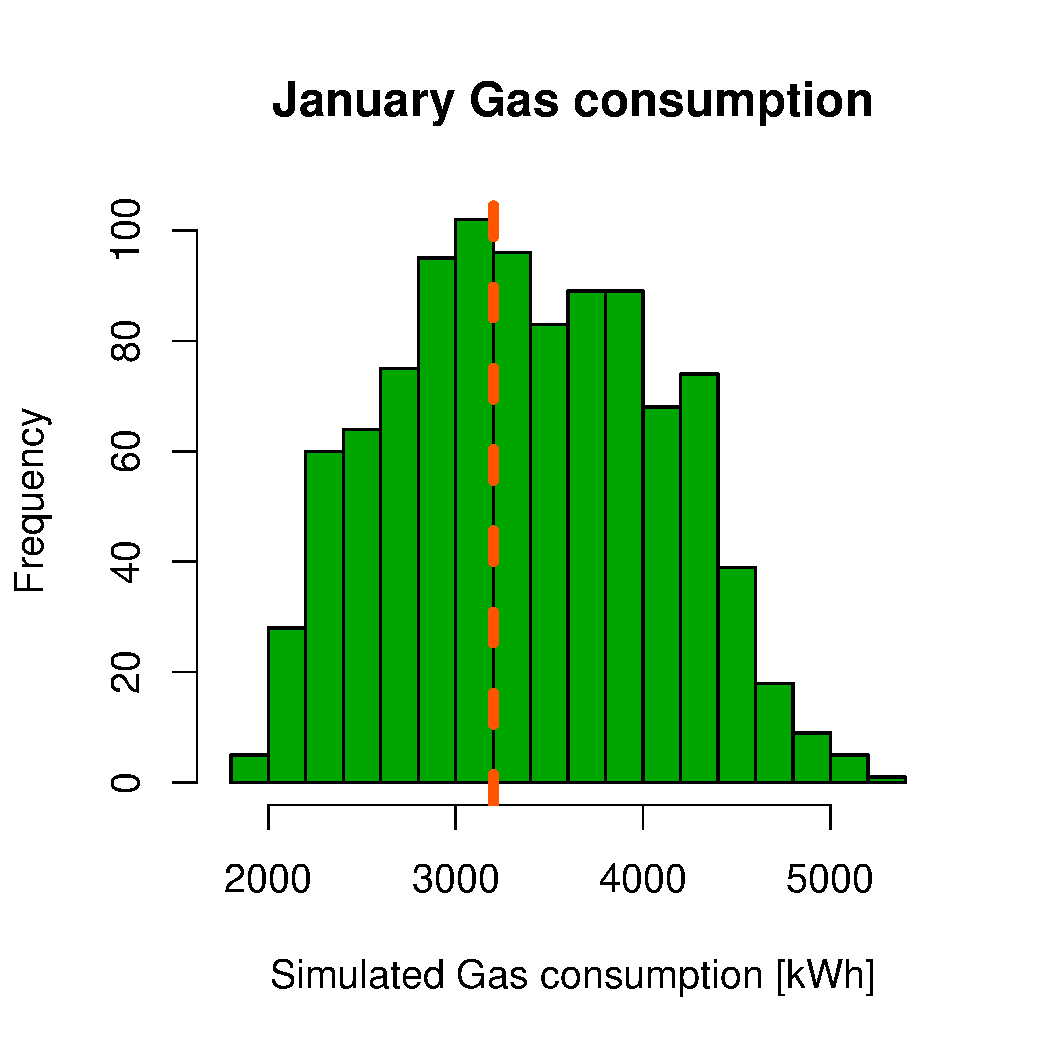
\includegraphics[width=\scale]{Simulation_histograms/Batch_2_Only/January_Gas}
 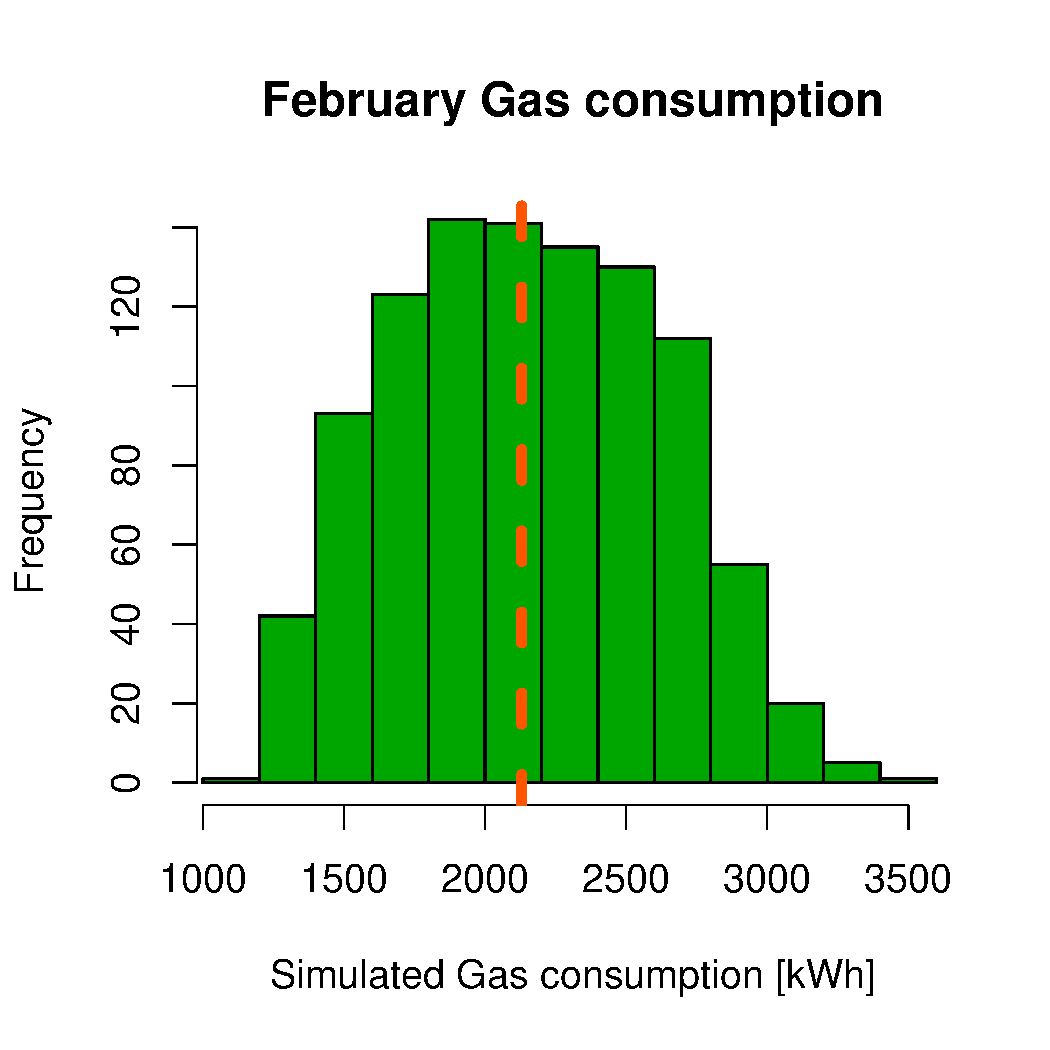
\includegraphics[width=\scale]{Simulation_histograms/Batch_2_Only/February_Gas}
 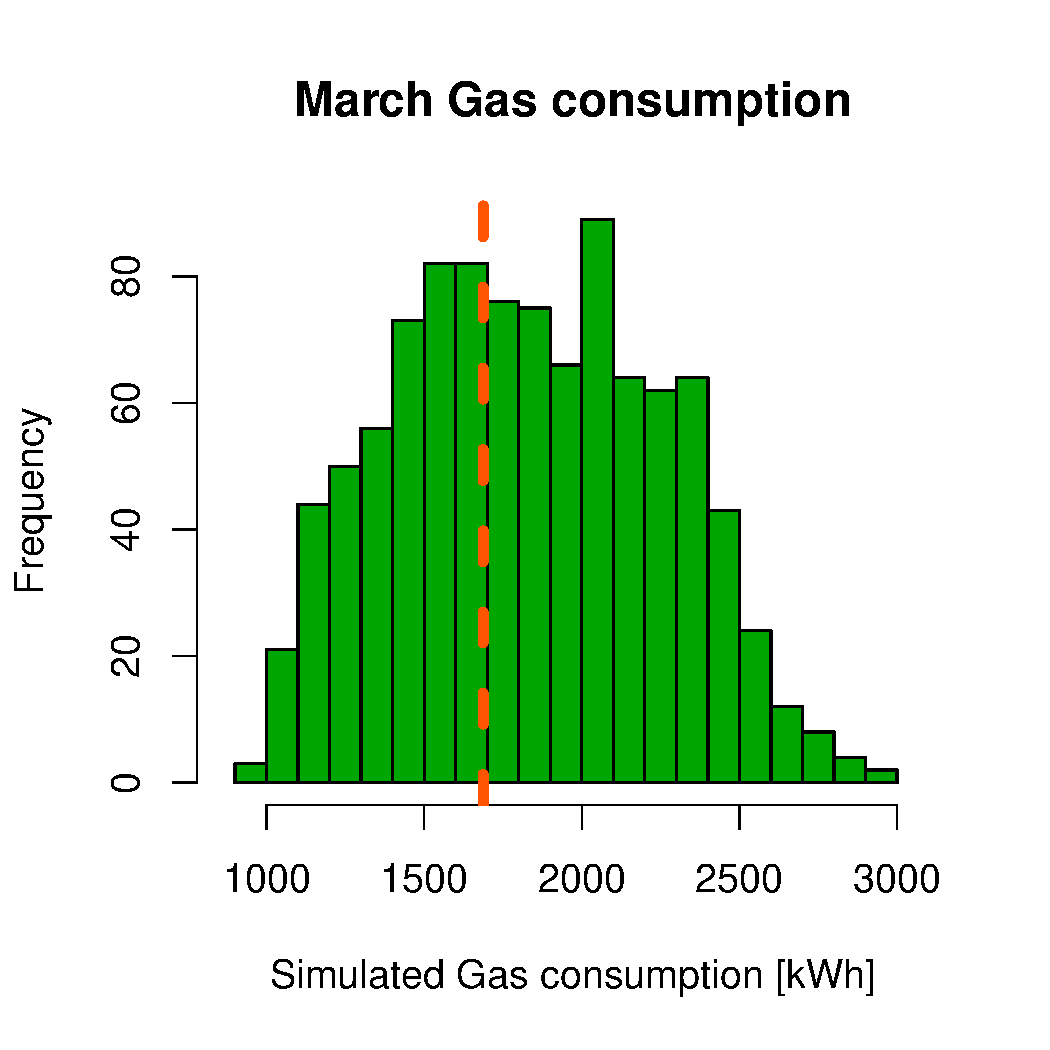
\includegraphics[width=\scale]{Simulation_histograms/Batch_2_Only/March_Gas}\\
 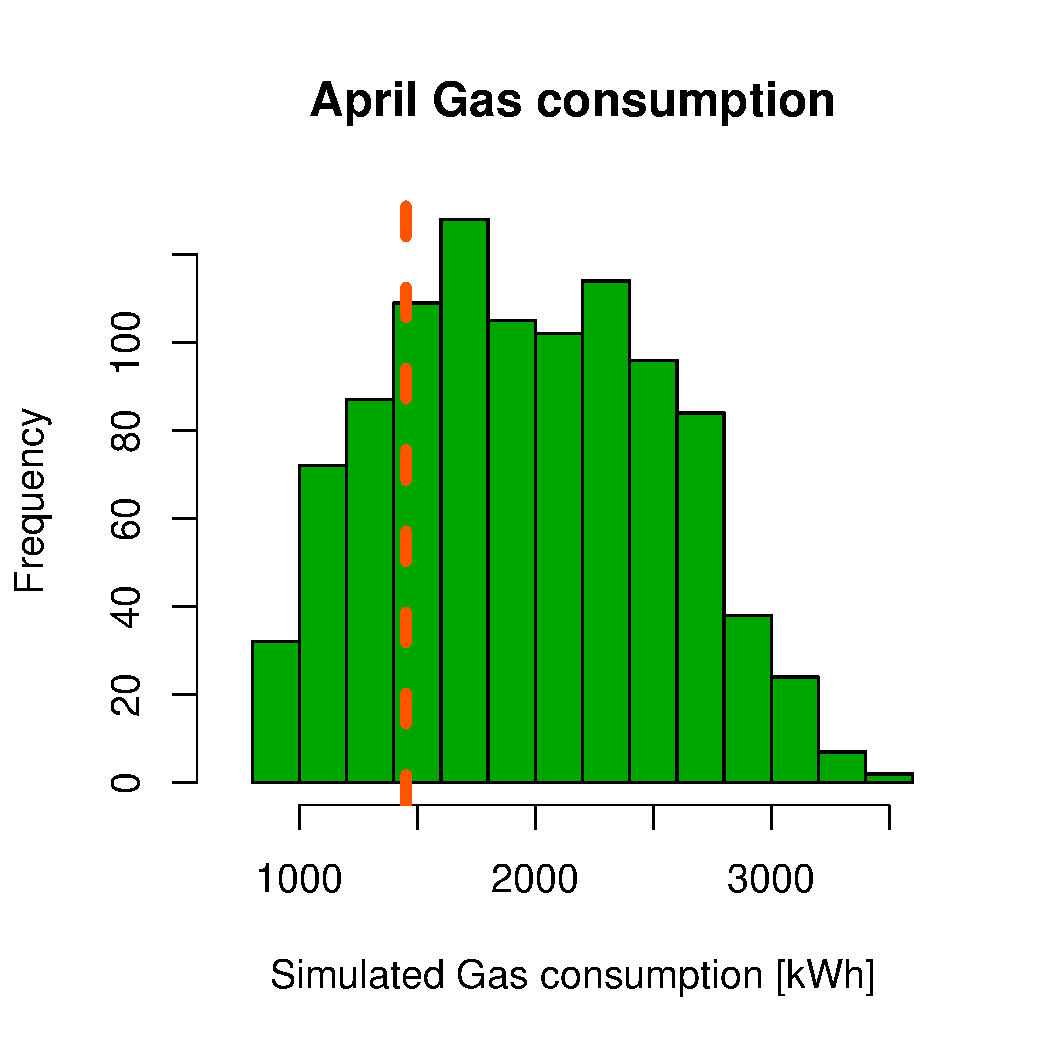
\includegraphics[width=\scale]{Simulation_histograms/Batch_2_Only/April_Gas}
 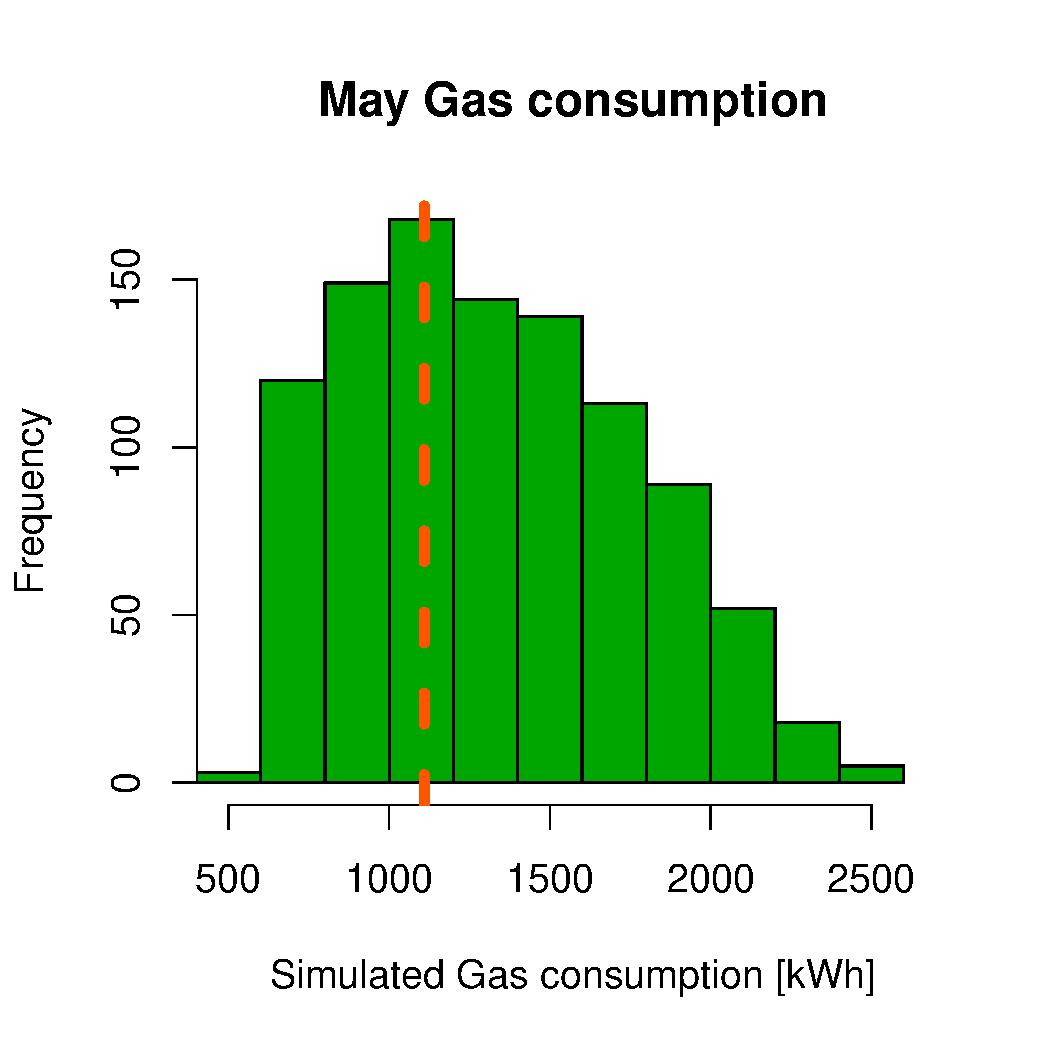
\includegraphics[width=\scale]{Simulation_histograms/Batch_2_Only/May_Gas}
 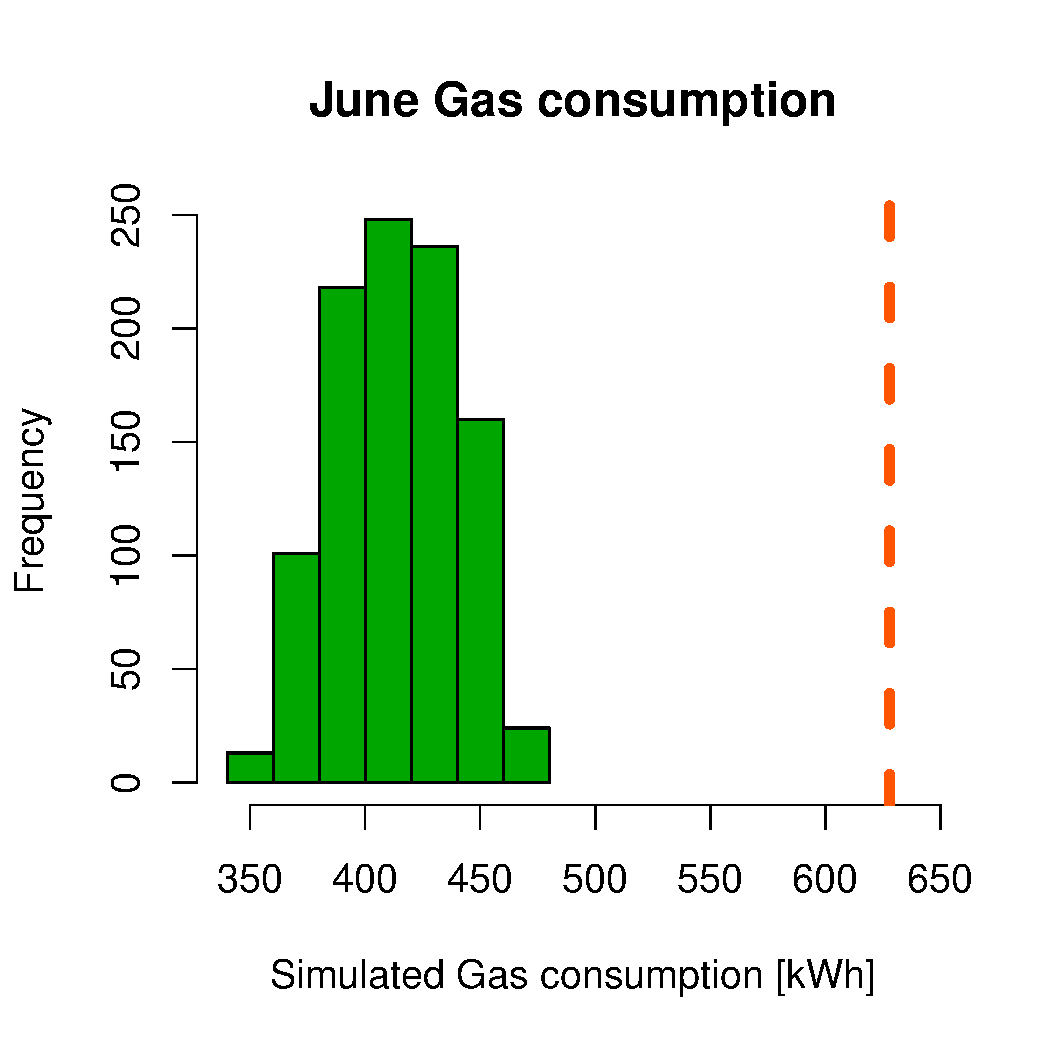
\includegraphics[width=\scale]{Simulation_histograms/Batch_2_Only/June_Gas}\\
 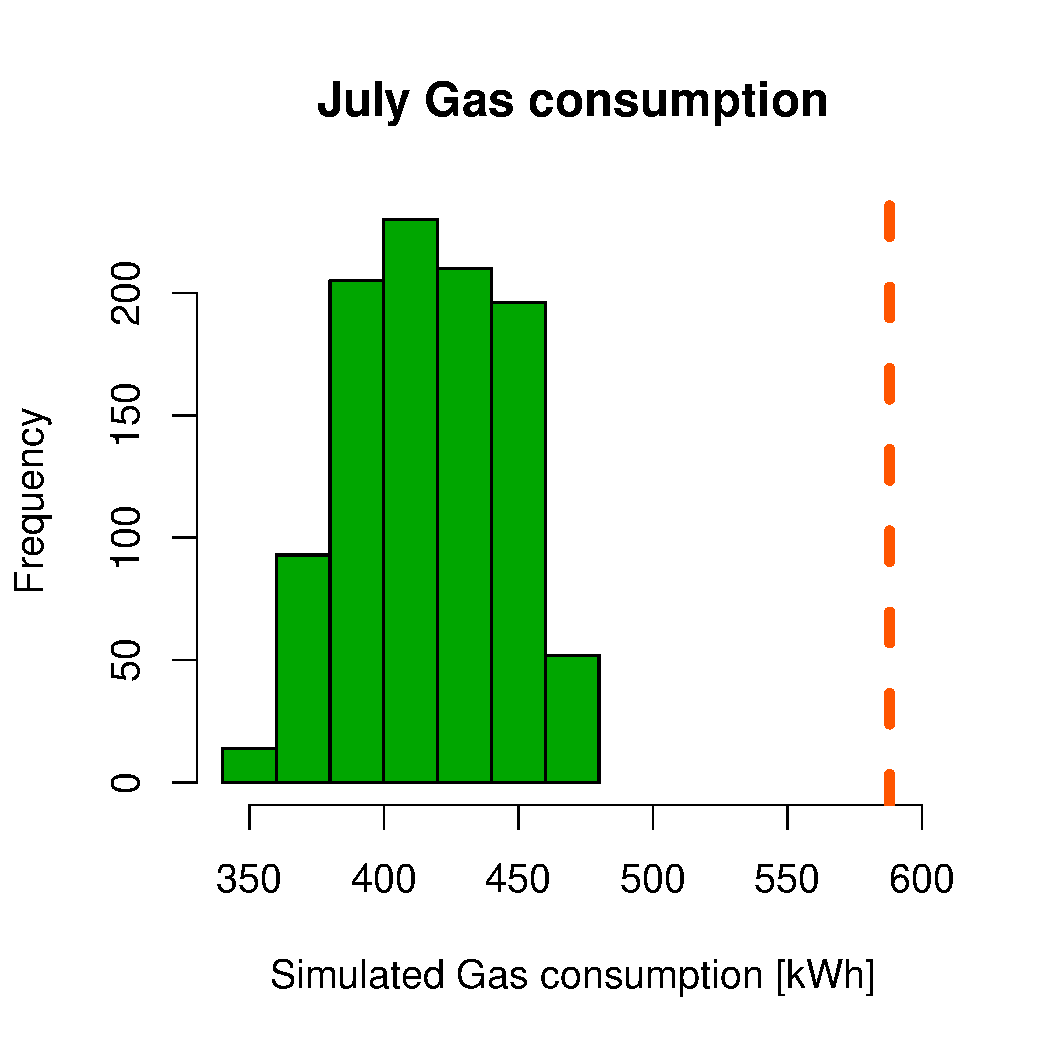
\includegraphics[width=\scale]{Simulation_histograms/Batch_2_Only/July_Gas}
 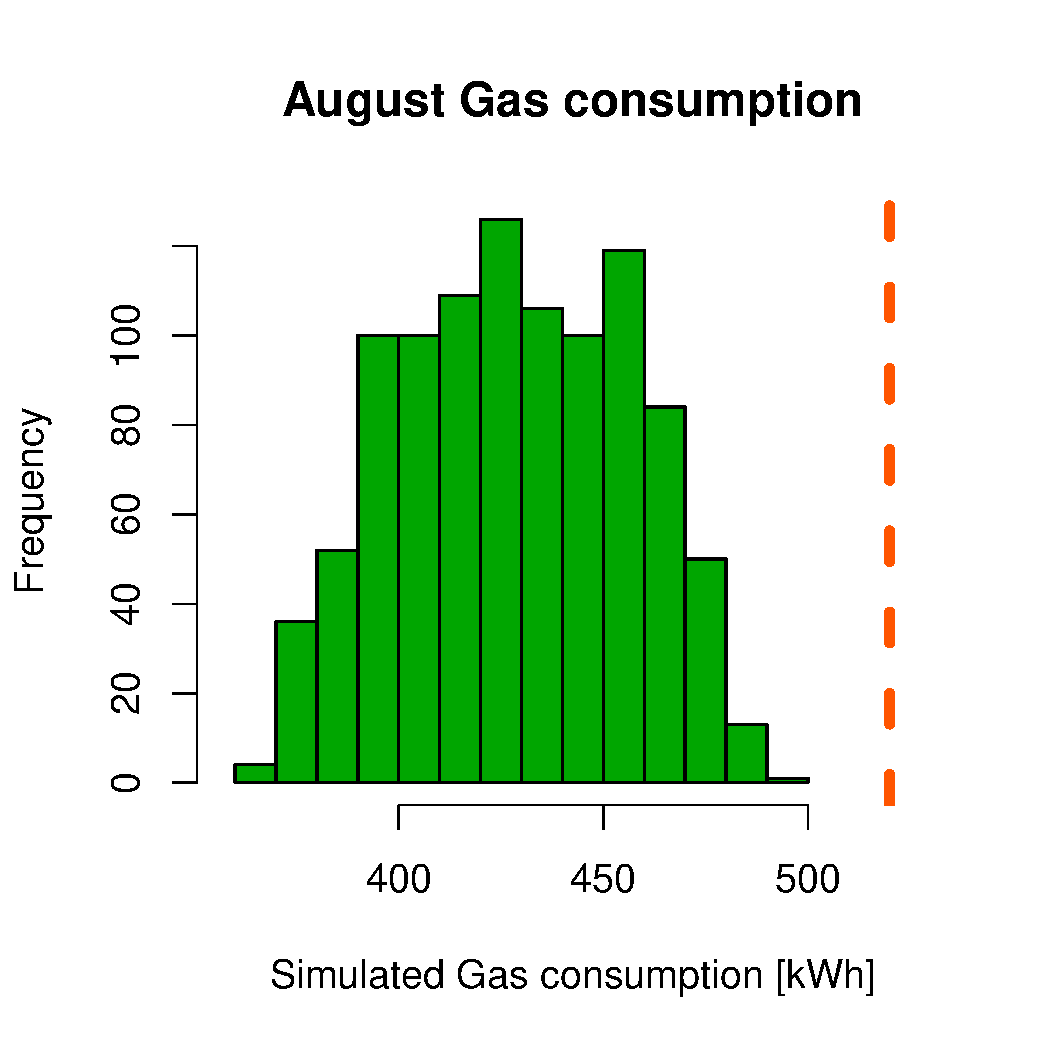
\includegraphics[width=\scale]{Simulation_histograms/Batch_2_Only/August_Gas}
 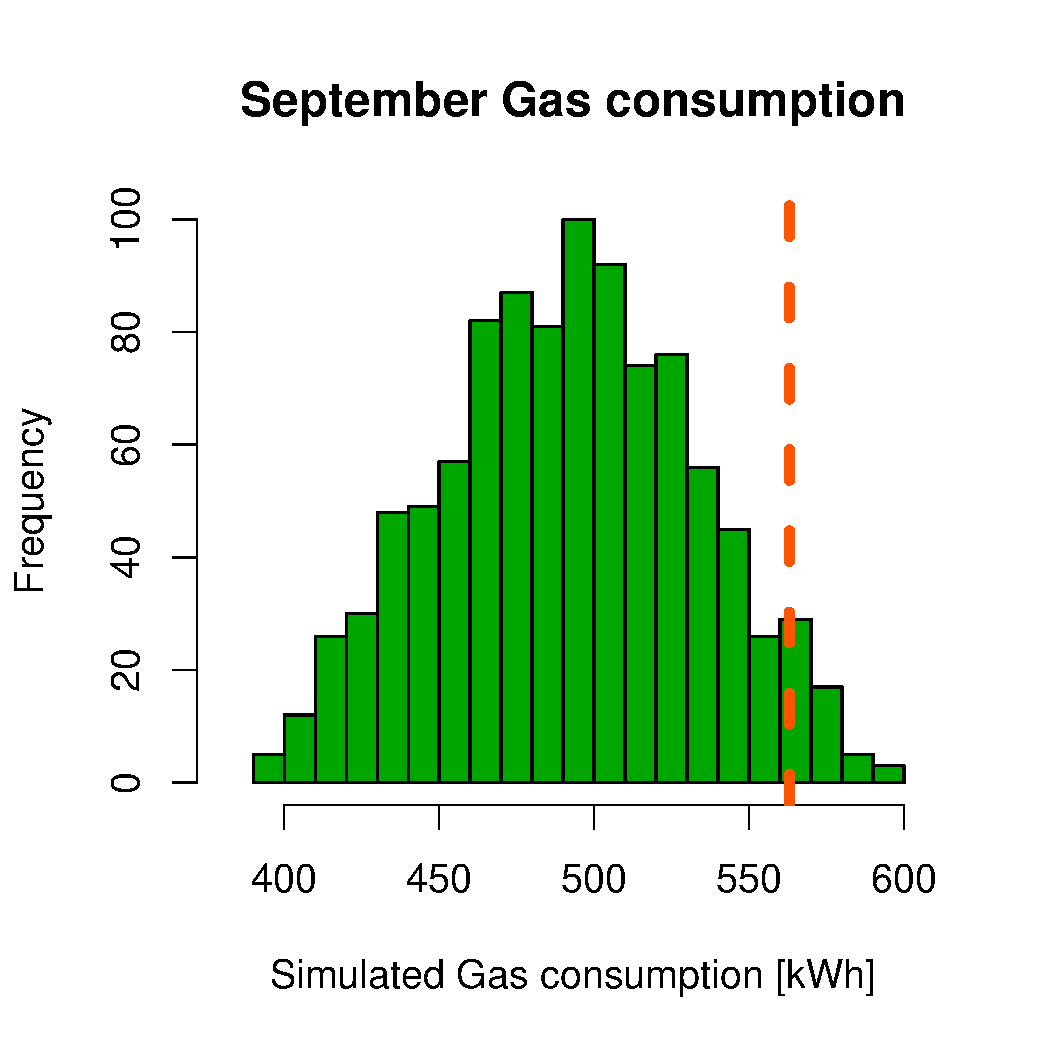
\includegraphics[width=\scale]{Simulation_histograms/Batch_2_Only/September_Gas}\\
 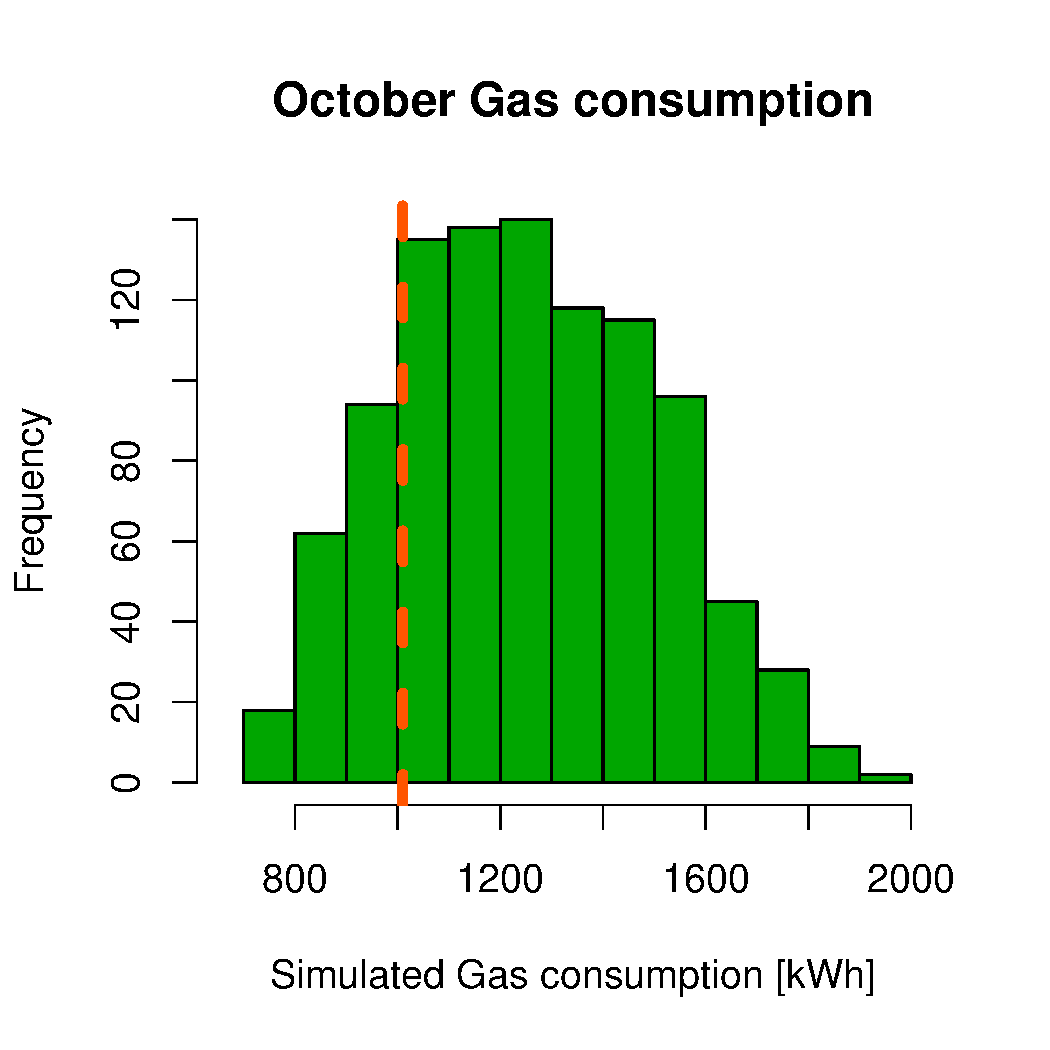
\includegraphics[width=\scale]{Simulation_histograms/Batch_2_Only/October_Gas}
 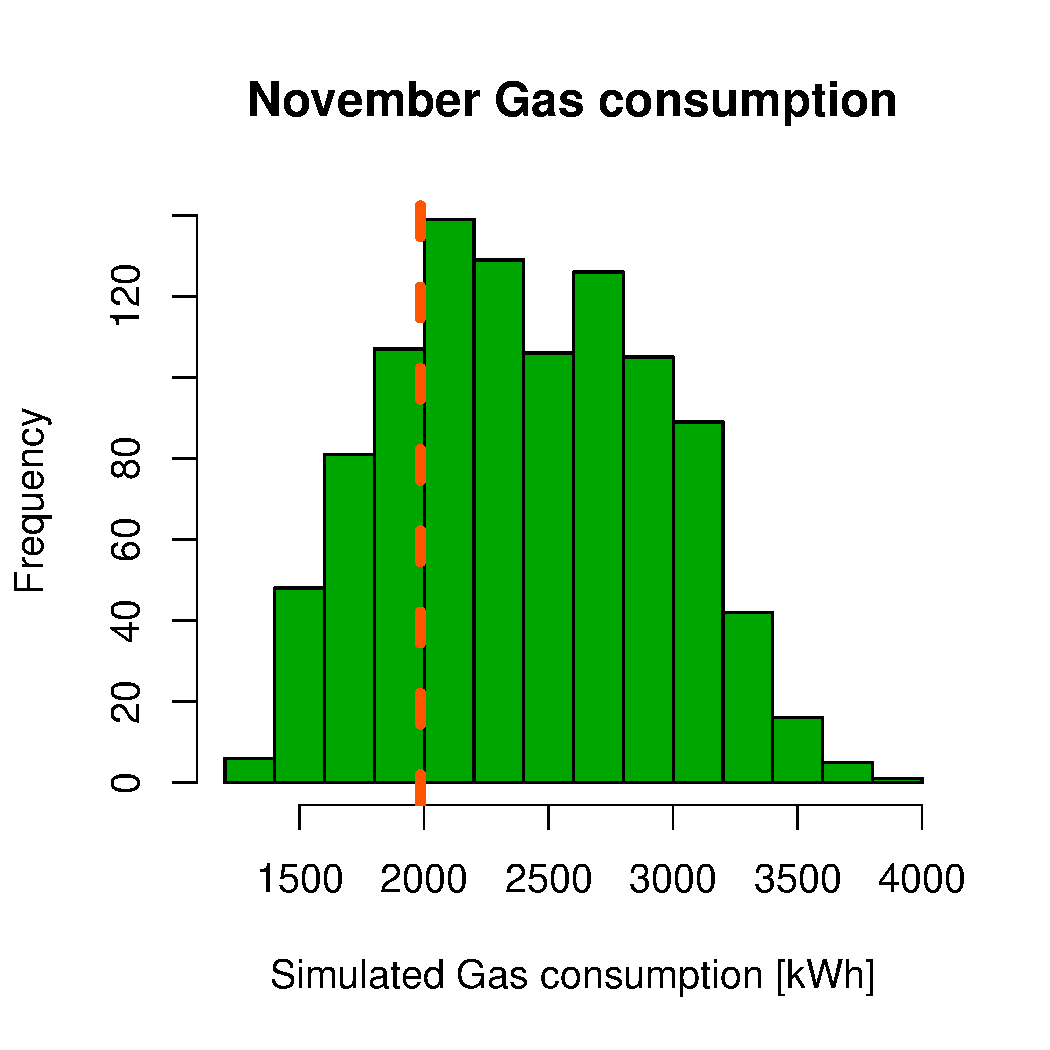
\includegraphics[width=\scale]{Simulation_histograms/Batch_2_Only/November_Gas}
 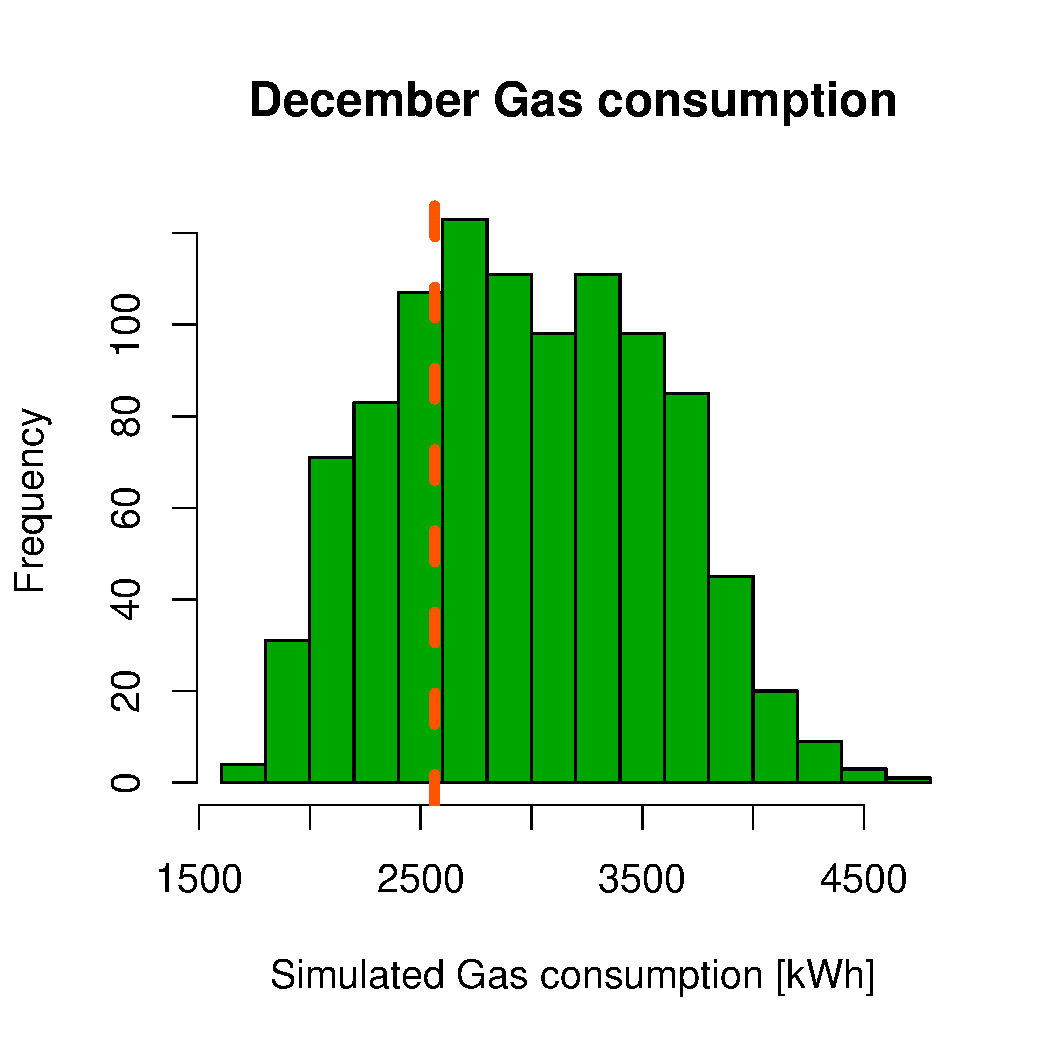
\includegraphics[width=\scale]{Simulation_histograms/Batch_2_Only/December_Gas}\\
 \caption{Distribution of the simulated monthly gas
 consumptions corresponding to the experimental design used in this work ($n=1000$ simulations).
 The $x$-value of the vertical dashed line in each plot locates the observed consumption for that month.}
 \label{Fig_Output_Hist}
\end{figure}


%%%%%%%%%%%%%%%%%%%%%%%%%%%%%%%%%%%%%%%%%%%%%%%%%%%%%%%%%%%%%%%%%%%%%%%%%%%%%%%%%



\section{Construction of the Emulators}\label{Sec_Emulators}

For each of the nine months we consider, it is natural to see the simulator as a function
\begin{equation*}
\begin{array}{l c c c}
 f \colon &  \R^8   & \longrightarrow & \R^+ \\
          &   \x  &     \mapsto     &  y
\end{array}.
\end{equation*}
To any choice $\x \in \R^8$ of the eight variables reported in \autoref{Table_Var_names}, the function associates the simulated gas consumption 
$y=f(\x)$ for that month.
In the following, we first set the notation and introduce the parameters which will need to be estimated in order to build an emulator of such a function (Section~\ref{Sec_General}). The procedure used to estimate/choose these parameters for each of the nine months of interest is detailed in Section~\ref{Sec_Choices}.

\subsection{General Setting}\label{Sec_General}
The $n=1000$ runs provide the value of the function $f(\cdot)$ at the design points, 
which we denote as $\bd{x_i} \in \R^8$, $i=1, \dots, n$.
Following the classical emulation approach, we model $f(\cdot)$ as a stochastic process, specifically in the following way:
\begin{equation}\label{f}
 f(\x) \,=\, \sum_{j=0}^r \beta_j \, g_j(\bd{x^\A}) \,+\, \eta(\bd{x^\A}) \,+\, \eps(\x) \,,
\end{equation}
where the first term (the sum) represents the mean of $f(\cdot)$, while the other two terms are both zero-mean stochastic processes which account for the local deviation of 
$f(\cdot)$ from its mean. More details follow.

\begin{itemize}
 \item The vector $\bd{x^\A} \in \R^p$, $p \leq 8$, is meant to denote the ``active''
       inputs of the function $f(\cdot)$, the ones which have a more notable effect in explaining the variability of $f(\cdot)$ across different runs. The mean of $f(\x)$ is a linear combination of functions of the active inputs $\xA$: these functions are the $g_j(\cdot)$, which we will refer to as regressors. The function $g_0(\cdot)$ will be chosen to be identically equal to 1, so the mean of $f(\x)$ is an affine combination of the regressors $g_1(\xA), \dots, g_r(\xA)$.
 \item The process $\eta(\cdot)$ is a zero-mean stochastic process, with 
       squared-exponential covariance function. That is (dropping for a moment the superscript $[A]$ for convenience), we have:
       \begin{equation}\label{Cov_fun}
         \text{Cov}\big[ \eta(\x), \eta(\x^\prime)  \big] = {\sigma_{\eta}}^2 \,
           \exp \left( 
              - \frac{1}{2} \; \sum_{k=1}^p \left(\frac{x_k - x^\prime_k}{d_k}\right)^2
           \; \right), 
           \quad\; \x, \x^\prime \in \R^p.
       \end{equation}
       This form assumes that the variance of $\eta(\cdot)$ is constant across the space, equal to ${\sigma_\eta}^2$. The values of both ${\sigma_\eta}^2$ and the correlation lengths $d_k$ will be set according to the case (Section~\ref{Sec_Choices}).
 \item The term $\eps(\x)$ represents a ``nugget'' term, accounting for the 
       residual local variability of $f(\cdot)$ not accounted for by the previous term. As it is usual, we model this as a zero-mean real stochastic process independent of $\eta(\cdot)$, with constant variance ${\sigma_\eps}^2$ and uncorrelated outputs at any two points of the space.
\end{itemize}

The previous specifications uniquely determine the mean and covariance structure of the process $f(\cdot)$ in \eqref{f}. In light of the simulation outputs
\begin{equation*}
 y_i = f(\bd{x_i}), \quad i=1, \dots, n,
\end{equation*}
we can use the linear Bayes methodology to adjust the mean and covariance specifications above. (I won't go into the details of presenting the formulas here, we'll do this for the paper instead, according to the journal we'll submit the work to).

\subsection{Specific Choices}\label{Sec_Choices}
This section provides the details of the specific choices made to build the nine emulators of this work (each associated with one of the non-summer months). In particular, it concerns the choices of the active inputs $\xA$, regressors $g_j(\cdot)$, correlation lengths $d_k$ and variances ${\sigma_\eta}^2$, ${\sigma_\eps}^2$. 


To select the active variables and the associated regressors, we consider a larger set of potential regressors formed by all linear, quadratic and interaction terms of the eight input variables (after linearly rescaling these onto the range $[-1,1]$). This yields a total of 44 potential regressors. Hence, for each integer $\Nr \leq 44$, among all linear models expressing $y_i$ as linear combination of exactly $\Nr$ regressors, we select the model with the greatest coefficient of determination $R^2$.
This procedure allows us to identify, for each integer $\Nr$, the set of $\Nr$ regressors of order at most 2 which best explain the set of simulated gas consumptions ${\{y_i\}}_{i=1, \dots, n}$.


The results of this procedure show that, for all nine months, the ``best'' five regressors are sufficient to explain more than $99\%$ of the output variance; in fact, with the only exception of September, four regressors are already sufficient to achieve the result. In spite of this already excellent fit, adding sequentially further regressors to the models, as per the above procedure, improves the models significantly. For all the nine months, and up to models with 13 regressors, the null hypothesis of a zero coefficient associated with any of the considered regressor is confidently rejected with a $p$-value lower than the machine epsilon ($\approx 10^{-16}$). 
In order to avoid a model with an excessive number of regressors, we use the procedure above to select the first 10 best regressors for each month, and use these as functions $g_1(\cdot), \dots, g_r(\cdot)$ in equation~\eqref{f}, with $r=10$ and $g_0(\cdot) \equiv 1$. An exception to this rule is represented by the emulator for the month of May: this is discussed further below.


Once the set of regressors for a given month has been chosen, we consider as active inputs the ones in the set $\{V_1, \dots, V_8\}$ which play an active role in the regressors. In a few cases, one variable $V_j$ not appearing in the expression of the selected regressors may have nonetheless been included in the set of active inputs: this is due to the fact that that variable does appear as significant in the corresponding linear regression model, as a term just beyond the tenth. It does therefore play an important role in explaining the structure of the regression residuals, through which we fit a stochastic process (the terms $ \eta(\cdot) + \eps(\cdot)$ in equation~\eqref{f}).
\autoref{Table_Regressors} shows the sets of regressors and active inputs selected for each month, alongside the adjusted $R^2$ of the associated linear regression.


\begin{table}
 \centering
 \renewcommand{\arraystretch}{1.4}
 \newcommand{\colsep}{3ex}
 \caption{For each of the nine months considered, in order from left to right: i) the list of regressors used as functions $g_j(\cdot)$ in equation~\eqref{f}; ii) the list of active inputs used to specify the covariance function in equation~\eqref{Cov_fun}; iii) the adjusted $R^2$ of the linear regression built with the regressors in column i).
 In this column, the ``$\ast$'' symbol is used as shorthand notation for all linear and interaction terms, \eg\ $\,a \ast b \ast c = 
 \{ a, b, c , ab, ac, bc \}$.}
% \small
 \begin{tabular}{c<{\hspace{\colsep}}  c<{\hspace{\colsep}}  c<{\hspace{\colsep}} c}
\specialrule{.1em}{0em}{0.1em} 
 \textbf{Month} &  \textbf{Regressors} & \textbf{Active Inputs} & \textbf{Adj.~$R^2$}\\
 \specialrule{.05em}{.1em}{0.1em} 
 \specialrule{.05em}{0em}{0.2em} 
  Jan  &  $V_1 \!\ast\! V_2 \!\ast\! V_6, \,V_3,\, V_4,\,{V_2}^2,\,{V_6}^2$   &  $V_1, \,V_2, \,V_3, \,V_4, \,V_6$        & 0.9998 \\
  Feb  &  $V_1 \!\ast\! V_2 \!\ast\! V_6, \,V_3,\, V_4,\,{V_2}^2,\, {V_6}^2$  &  $V_1, \,V_2, \,V_3, \,V_4, \,V_6$        & 0.9998 \\
  Mar  &  $V_1 \!\ast\! V_2 \!\ast\! V_6, \,V_3,\, V_4,\,{V_2}^2,\, {V_6}^2$  &  $V_1, \,V_2, \,V_3, \,V_4, \,V_6, \,V_7$ & 0.9997 \\
  Apr  &  $V_1 \!\ast\! V_2 \!\ast\! V_6, \,V_3,\, V_4,\,{V_2}^2,\, {V_6}^2$  &  $V_1, \,V_2, \,V_3, \,V_4, \,V_6$        & 0.9998 \\  
  May  &  $V_1 \!\ast\! V_2 \!\ast\! V_6, \,V_3,\, V_8,\,{V_6}^2,\, V_1 {V_6}^2, \, {V_6}^3$  &  $V_1, \,V_2, \,V_3, \,V_6, \,V_8$ & 0.9991 \\
  Sep  &  $V_1 \!\ast\! V_2 \!\ast\! V_6, \,V_3,\, V_4,\, V_8,\, {V_6}^2$     &  $V_1, \,V_2, \,V_3, \,V_4, \,V_6, \,V_8$ & 0.9994 \\
  Oct  &  $V_1 \!\ast\! V_2 \!\ast\! V_6, \,V_3,\, V_4,\, V_8,\, {V_6}^2$     &  $V_1, \,V_2, \,V_3, \,V_4, \,V_6, \,V_8$ & 0.9996 \\
  Nov  &  $V_1 \!\ast\! V_2 \!\ast\! V_6, \,V_3,\, V_4,\,{V_2}^2,\, {V_6}^2$  &  $V_1, \,V_2, \,V_3, \,V_4, \,V_6, \,V_8$ & 0.9998 \\
  Dec  &  $V_1 \!\ast\! V_2 \!\ast\! V_6, \,V_3,\, V_4,\,{V_2}^2,\, {V_6}^2$  &  $V_1, \,V_2, \,V_3, \,V_4, \,V_6$        & 0.9998 \\
 \specialrule{.1em}{0.2em}{1em} 
 \end{tabular}
\label{Table_Regressors}
\end{table}

As mentioned previously, a slightly different procedure has been used to select the regressors and active inputs for the month of May. For this month, the plot of the linear regression residuals (linear model built as above with the best 10 regressors of order 2) against $V_1$ and especially $V_6$ showed a remarkable pattern, resembling the one of a polynomial of order higher than 2.
In light of this, before running the above linear regression procedure, we include all cubic terms involving either $V_1$ or $V_6$ 
in the set of potential regressors. Within the first 11 terms, both the cubic term in $V_6$ and the interaction term between $V_1$ and ${V_6}^2$ are picked by the procedure. This inclusion makes the relationship between the new model residuals and the two input variables much less obvious to interpret. We therefore consider this set of 11 regressors for May, and choose the variables appearing in them as active inputs. See \autoref{Table_Regressors} for details.



Once the regressors and active inputs are chosen for all the months, values for the correlation lengths $d_k$ and the two ``prior'' variances ${\sigma_\eta}^2, {\sigma_\eps}^2$ have to be set in order to build an emulator. 
As seen by equation~\eqref{f}, the quantity $ {\sigma_\eta}^2 + {\sigma_\eps}^2$ accounts for the local variability displayed by $f(\cdot)$ once the mean has been removed. For this reason, we impose:
\begin{equation}
 {\sigma_\eta}^2 + {\sigma_\eps}^2 = \sigma^2\,, \vspace{1.5ex}
\end{equation}
where $\sigma^2$ is the residuals' variance of the linear model used to select the regressors in $f(\cdot)$. Specifically, we impose that $95\%$ of the total variability $\sigma^2$ is ascribed to the ``structured'' process $\eta(\cdot)$ and the remaining $5\%$ to the ``random  noise'' process $\eps(\cdot)$:\vspace{0.7ex}
\begin{equation}
 {\sigma_\eta}^2 = 0.95 \,\sigma^2\,, \qquad {\sigma_\eps}^2 = 0.05 \,\sigma^2\,.\vspace{0.5ex}
\end{equation}


\begin{table}
 \centering
 \renewcommand{\arraystretch}{1.4}
 \setlength{\tabcolsep}{1.85ex}
 \caption{Month by month, values of the correlation length $d$ ($=d_1 =\dotso = d_p$) used in the squared-exponential covariance function \eqref{Cov_fun}, and of the residuals' standard deviation of the linear model built with the regressors in \autoref{Table_Regressors}.}
 \begin{tabular}{c<{\hspace{1ex}} ccccccccc}
  \specialrule{0.1em}{0em}{0.1em}
   & \textbf{Jan} & \textbf{Feb} & \textbf{Mar} & \textbf{Apr} & \textbf{May} 
   & \textbf{Sep} & \textbf{Oct} & \textbf{Nov} & \textbf{Dec} \\ 
 \specialrule{.05em}{.1em}{0.1em} 
 \specialrule{.05em}{0em}{0.2em} 
           $d$          & 0.35 &  0.3 & 0.35 &  0.3 &  0.4  &  0.4 & 0.45 &  0.5 & 0.35 \\
 $\sigma$ {\small[kWh]} & 9.26 & 7.25 & 7.19 & 7.11 & 12.69 & 0.96 & 4.91 & 7.59 & 8.26 \\
 \specialrule{.1em}{0.2em}{1em} 
 \end{tabular}
 \label{Table_d_sigma}
\end{table}

\enlargethispage{-1\baselineskip}
As far as the correlation lengths $d_k$ are concerned ($k=1, \dots, p$, equation~\eqref{Cov_fun}), in this first stage we make the simplifying assumption that, for a given month, they are all equal to each other:
\begin{equation}
 d_1 = \dotso =d_p = d\,.\vspace{1.5ex}
\end{equation}
For a fixed number $p$ of terms in equation~\eqref{Cov_fun}, increasing the value of $d$ leads to an increase in the correlation between different outputs of the process $\eta(\cdot)$. Notice, however, that for a fixed $d$ the correlation decreases if more terms are accounted for in the sum of equation~\eqref{Cov_fun}. According to the month considered and to the number of active inputs $p$, we choose a value of $d$ in the range $[0.3, 0.5]$. 
\autoref{Table_d_sigma} reports the specific choices of $d$ for each month, alongside the value $\sigma^2$ used as prior variance for the model.
The predictive ability of the emulators built with the parameters detailed in this section is tested via leave-one-out cross-validation, as the next section explains.


\subsection{Validation of the Emulators}
The emulators built via the choices detailed in Section~\ref{Sec_Choices} are validated via leave-one-out cross-validation. 
The method consists in training an emulator, with the choices of the previous section, on all pairs $(\bd{x_i}, y_i)$ but one, and then using the emulator to predict the output associated with the left-out input point. By leaving out all pairs in turn and comparing the emulator prediction to the known output, we can assess the predictive ability of the emulator. 


Suppose the pair $(\bd{x_i}, y_i)$ is left out from the training set of the emulator. Let $\widehat y_i$ and $\widehat\sigma_i$ be the emulator mean prediction and standard deviation at the point $\bd{x_i}$, respectively. The following quantity:
\begin{equation}\label{Eqn_St_Err}
 \widehat{\eps}_i = \frac{\, \widehat y_i - y_i \,}{\widehat \sigma_i}
\end{equation}
measures the distance between the emulator prediction and the real simulator output $y_i$, in multiples of the emulator standard deviation. We therefore call $\,\widehat \eps_i$ the (cross-validated) standardised error for the $i^\text{th}$ data point.
Under Pukelsheim $3\sigma$-rule, a well-calibrated emulator would show at least $95\%$ of the $\widehat \eps_i$ to be in modulus smaller than 3. %The result would hold true with a threshold lower than 3  under specific distributional assumptions on the emulator, \eg\ Gaussianity: our approach, however, is general and does not require any such assumption to work.
\vspace{-1ex}

\autoref{Fig_Histograms_Errors} shows, for each of the months of interest, the distribution of the $n=1000$ standardised errors. The histograms suggest that all nine emulators are able to provide accurate predictions and correctly assess the uncertainty of these.
In addition, in \autoref{Fig_Scatter_Errors} we show the plots of the same set of standardised errors against the emulator fitted values. The plots aim to assess whether the errors' distribution is mostly coherent across the different $\widehat y_i$ values. Most of the plots confirms that this is the case. In a few rare cases (\eg, April), the magnitude of the standardised errors may be higher near the edges of the range of simulated values. Overall, the plots show nonetheless a satisfactory fit, especially for values $\widehat y_i$ in a neighbourhood of the observed gas consumption for that month: this is represented as a vertical orange dashed line in each panel.


\renewcommand{\scale}{13.2em}
\begin{figure}
\centering
 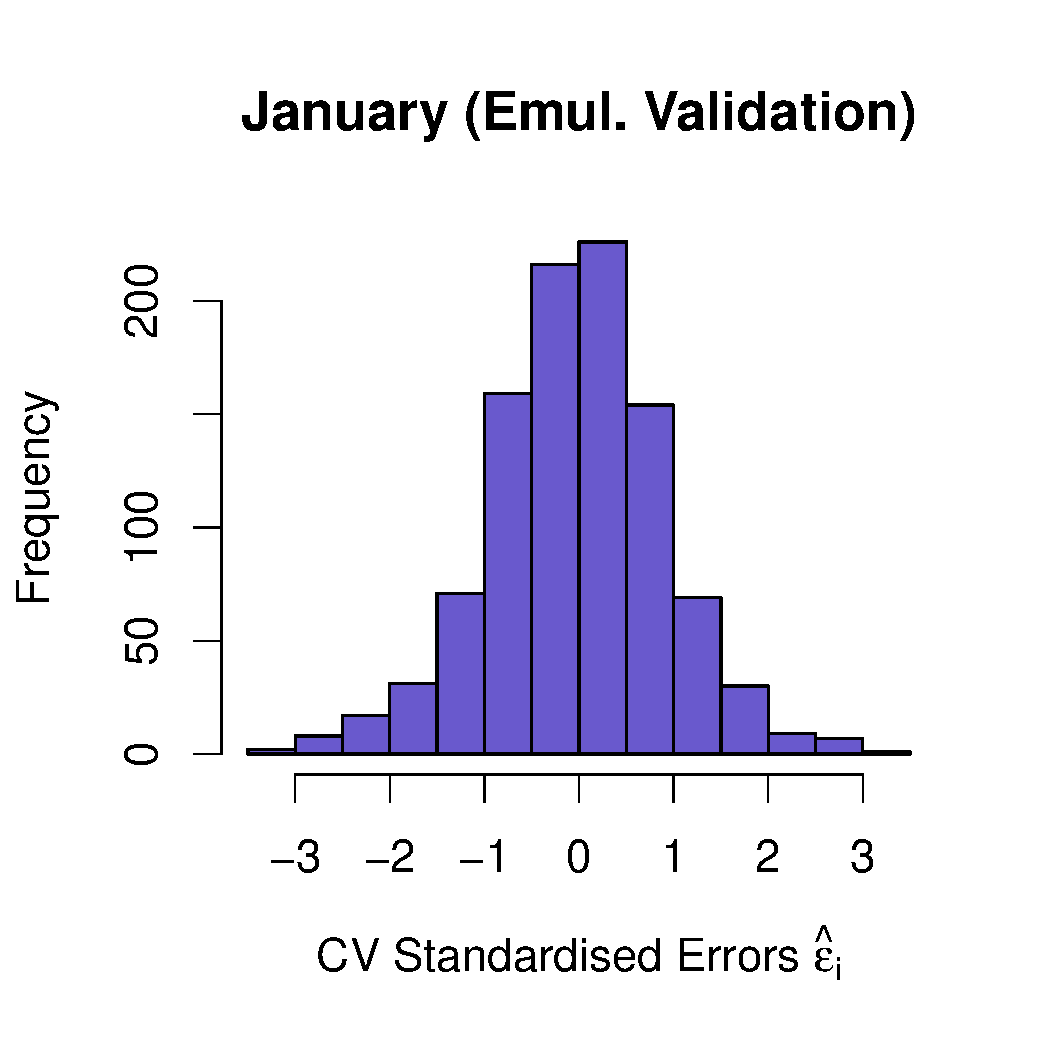
\includegraphics[width=\scale]{Emulator_CV/Histograms/January_CV_Errors_Hist}\hspace{-3ex}
 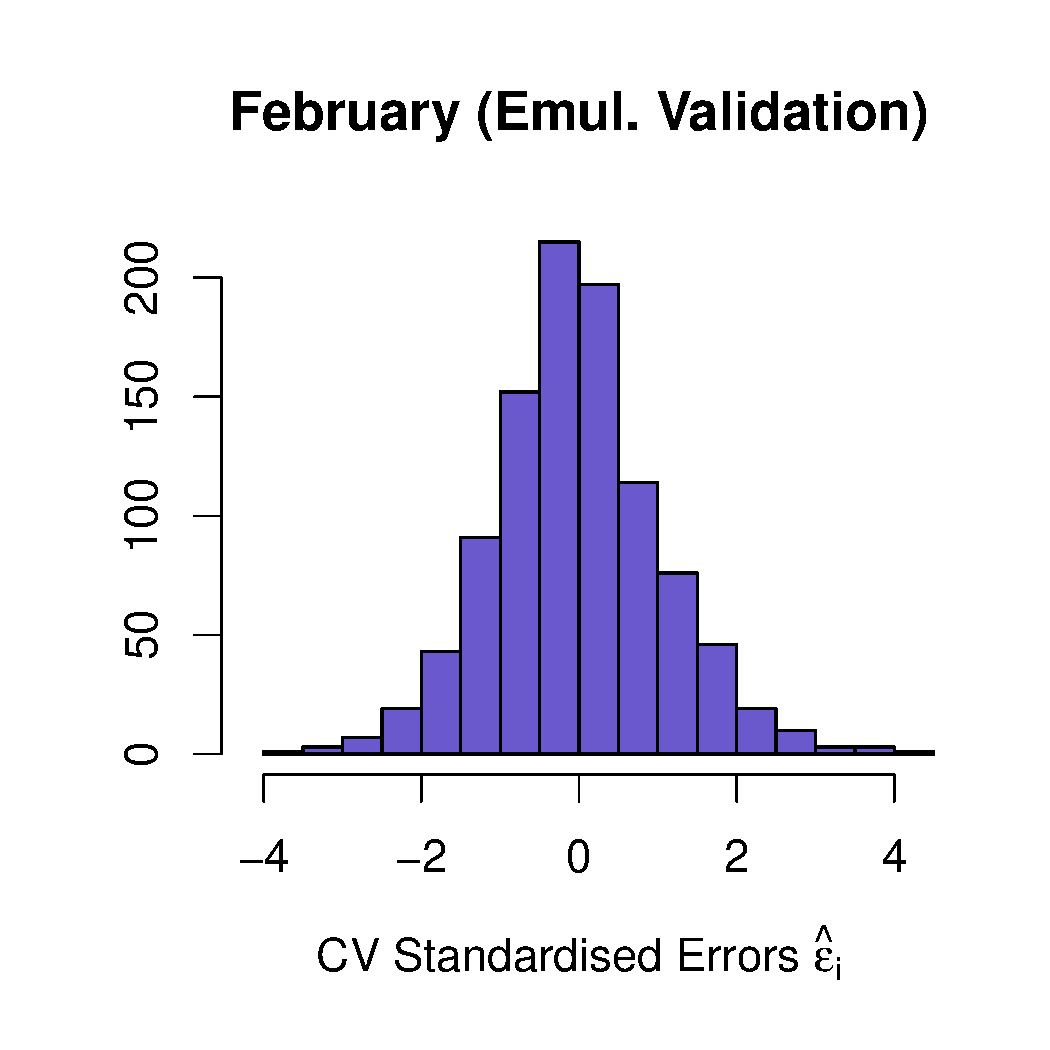
\includegraphics[width=\scale]{Emulator_CV/Histograms/February_CV_Errors_Hist}\hspace{-3ex}
 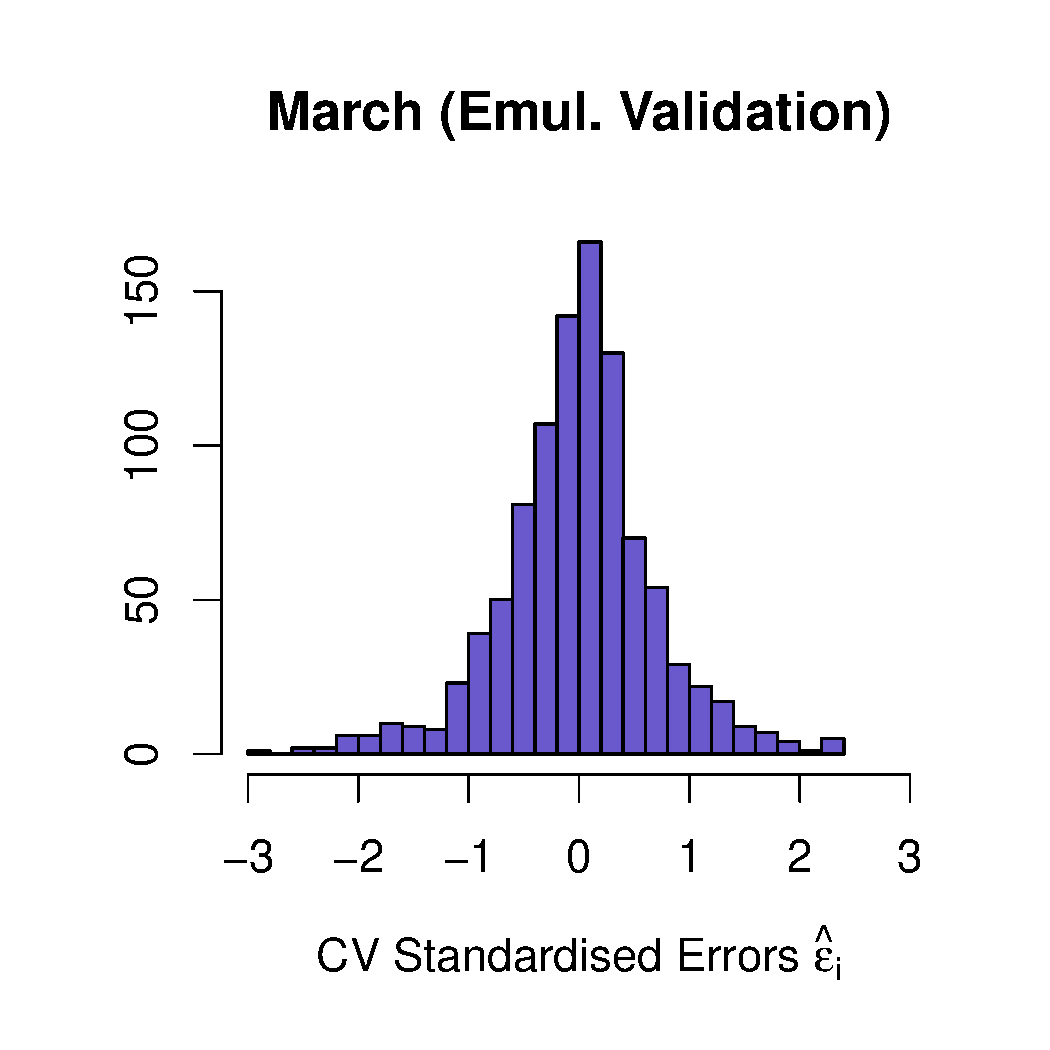
\includegraphics[width=\scale]{Emulator_CV/Histograms/March_CV_Errors_Hist}\\[-1ex]
 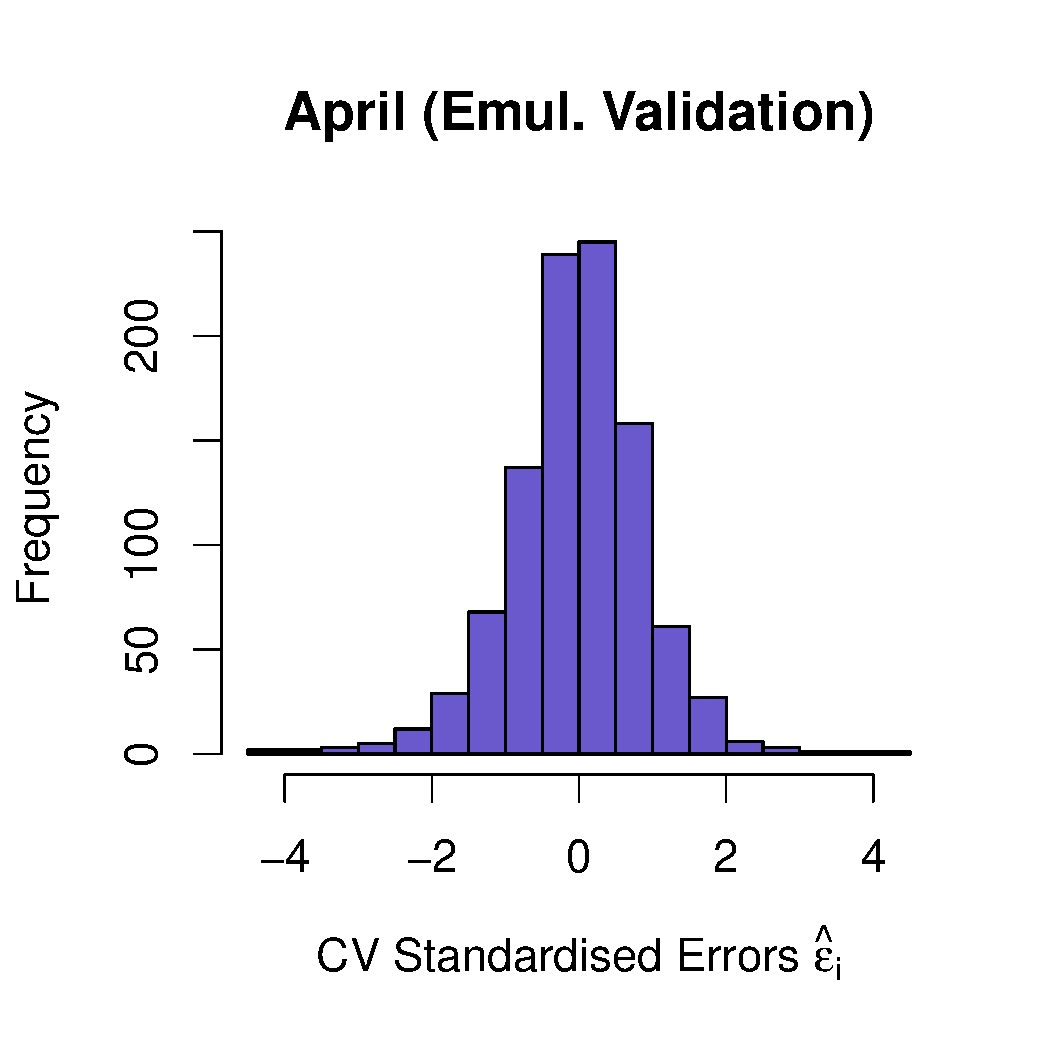
\includegraphics[width=\scale]{Emulator_CV/Histograms/April_CV_Errors_Hist}\hspace{-3ex}
 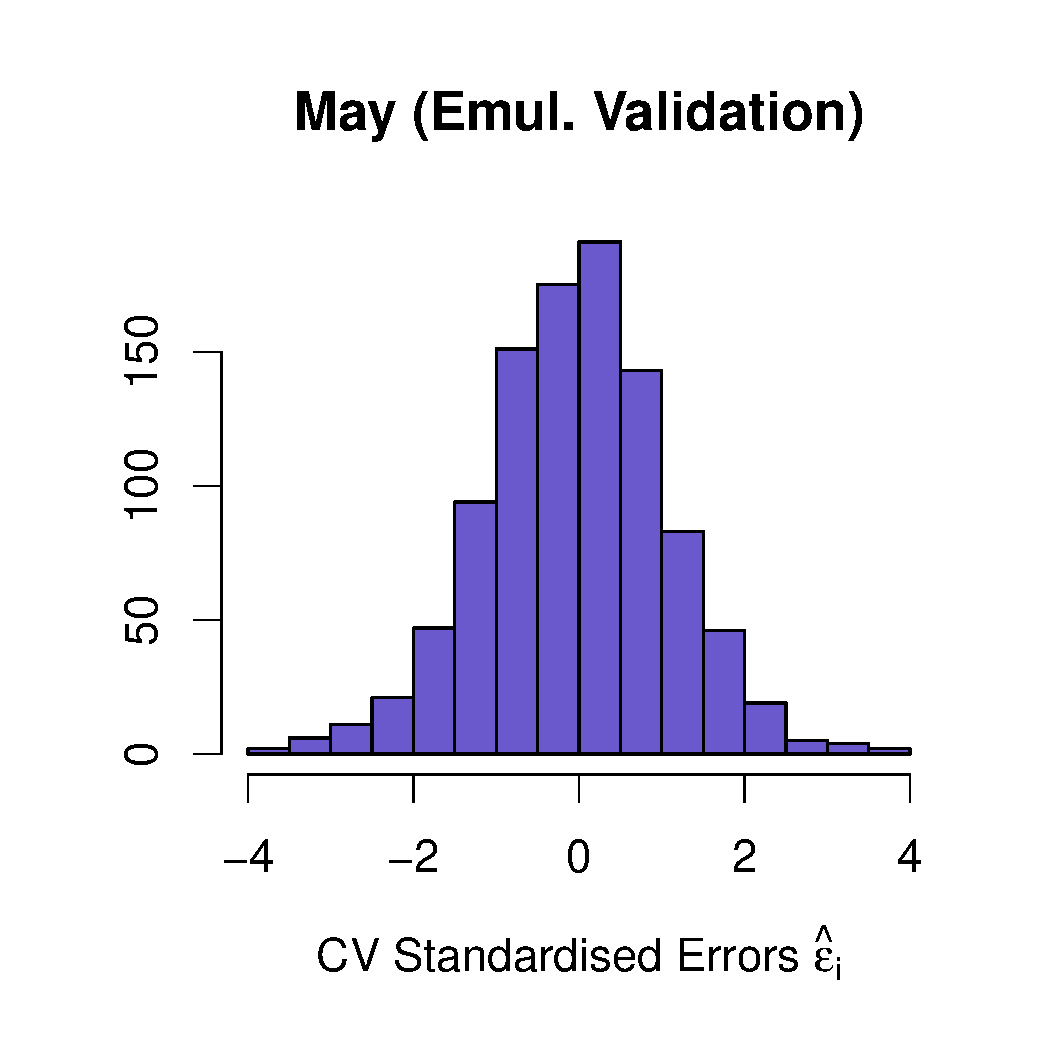
\includegraphics[width=\scale]{Emulator_CV/Histograms/May_CV_Errors_Hist}\hspace{-3ex}
 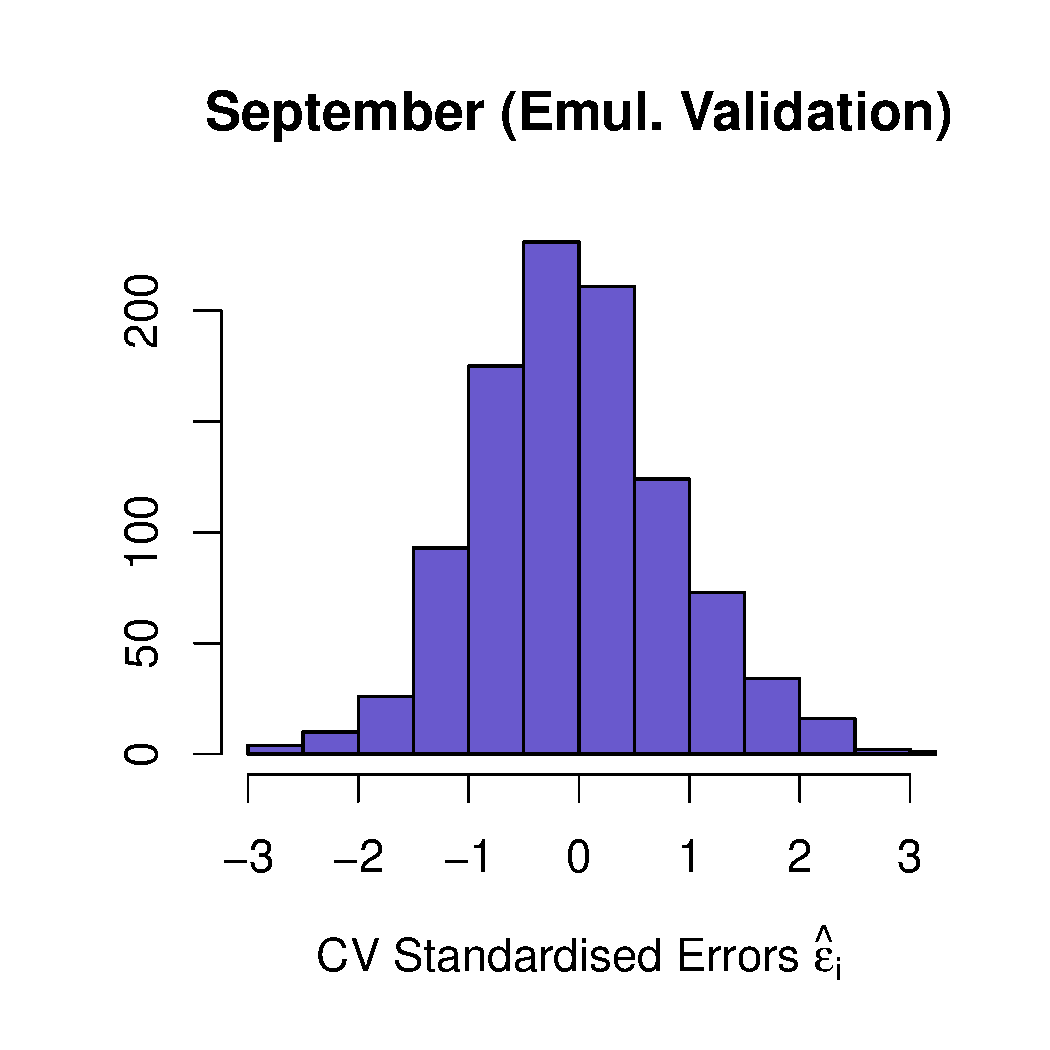
\includegraphics[width=\scale]{Emulator_CV/Histograms/September_CV_Errors_Hist}\\[-1ex]
 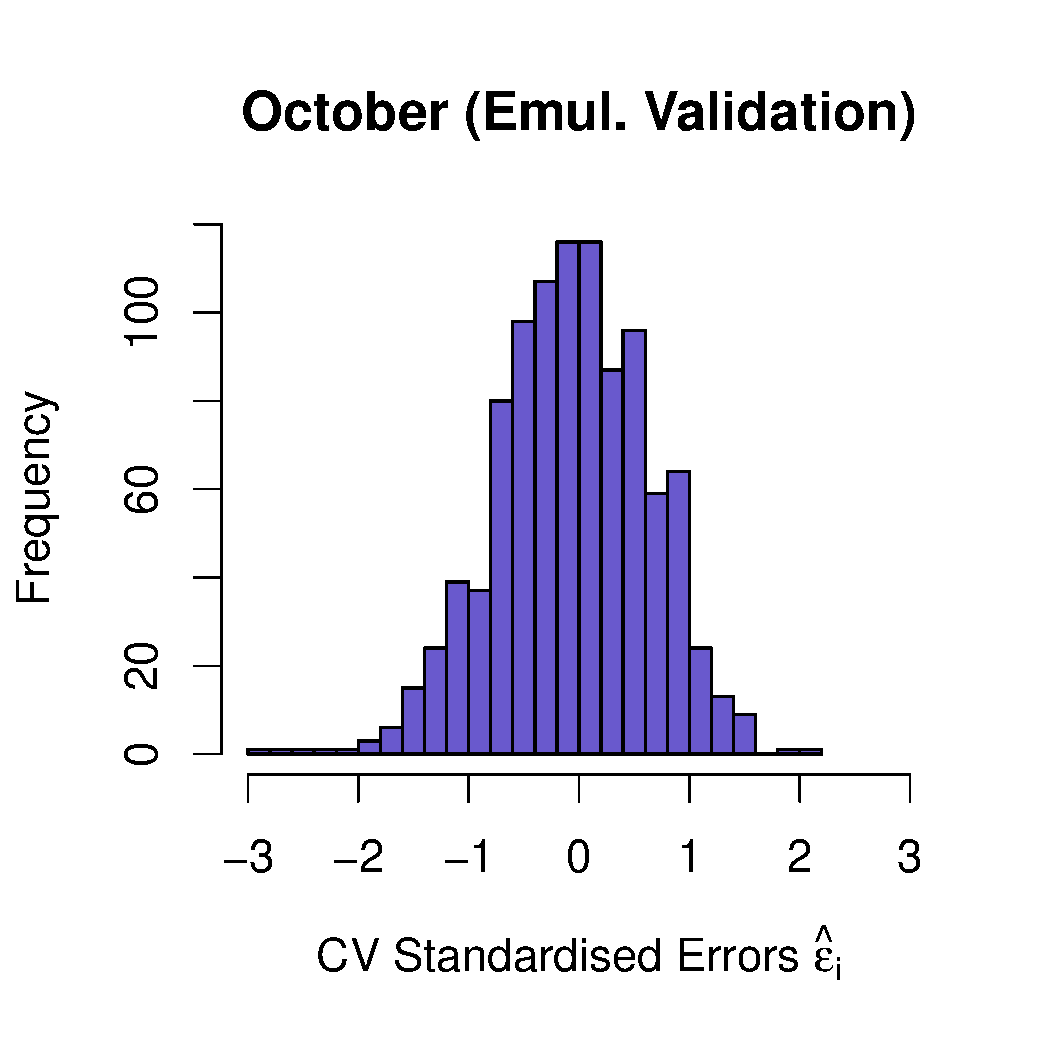
\includegraphics[width=\scale]{Emulator_CV/Histograms/October_CV_Errors_Hist}\hspace{-3ex}
 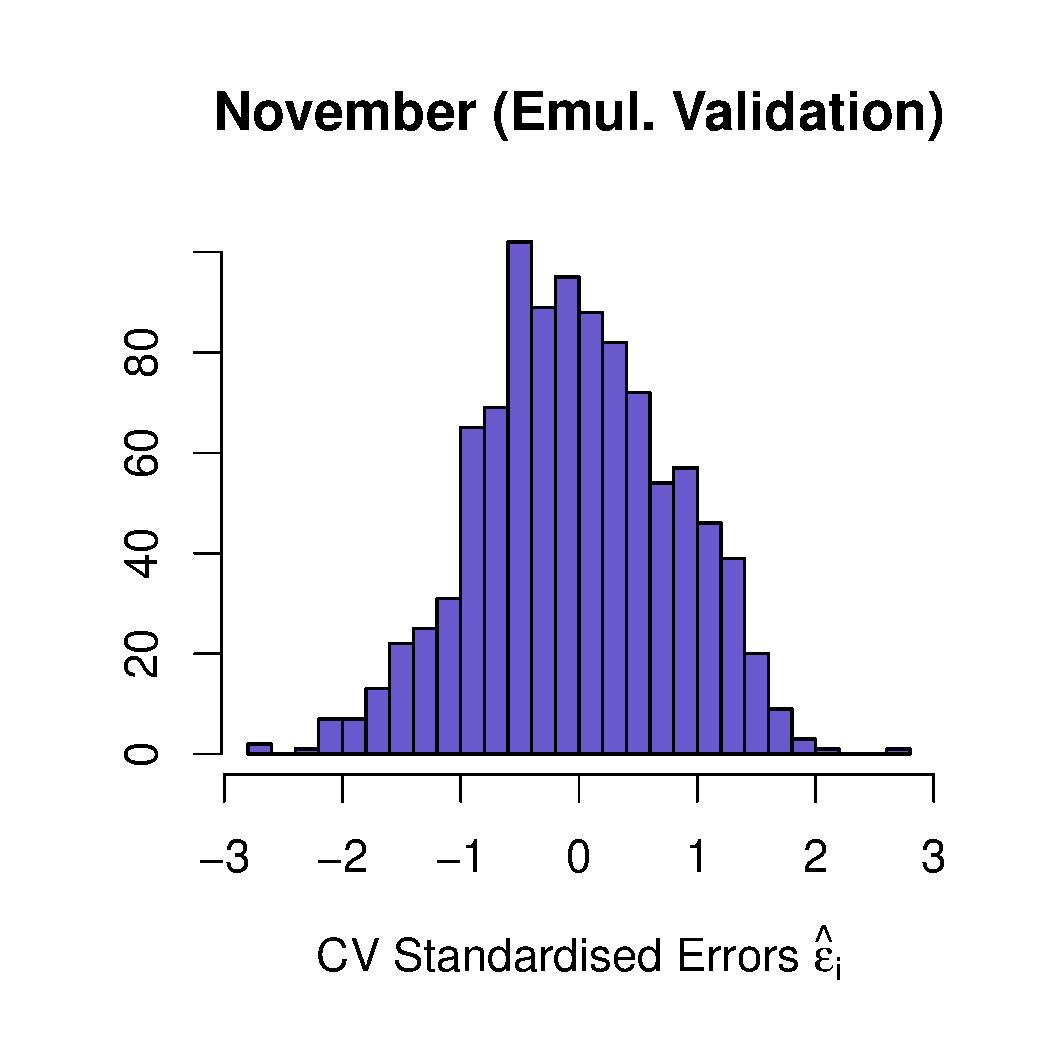
\includegraphics[width=\scale]{Emulator_CV/Histograms/November_CV_Errors_Hist}\hspace{-3ex}
 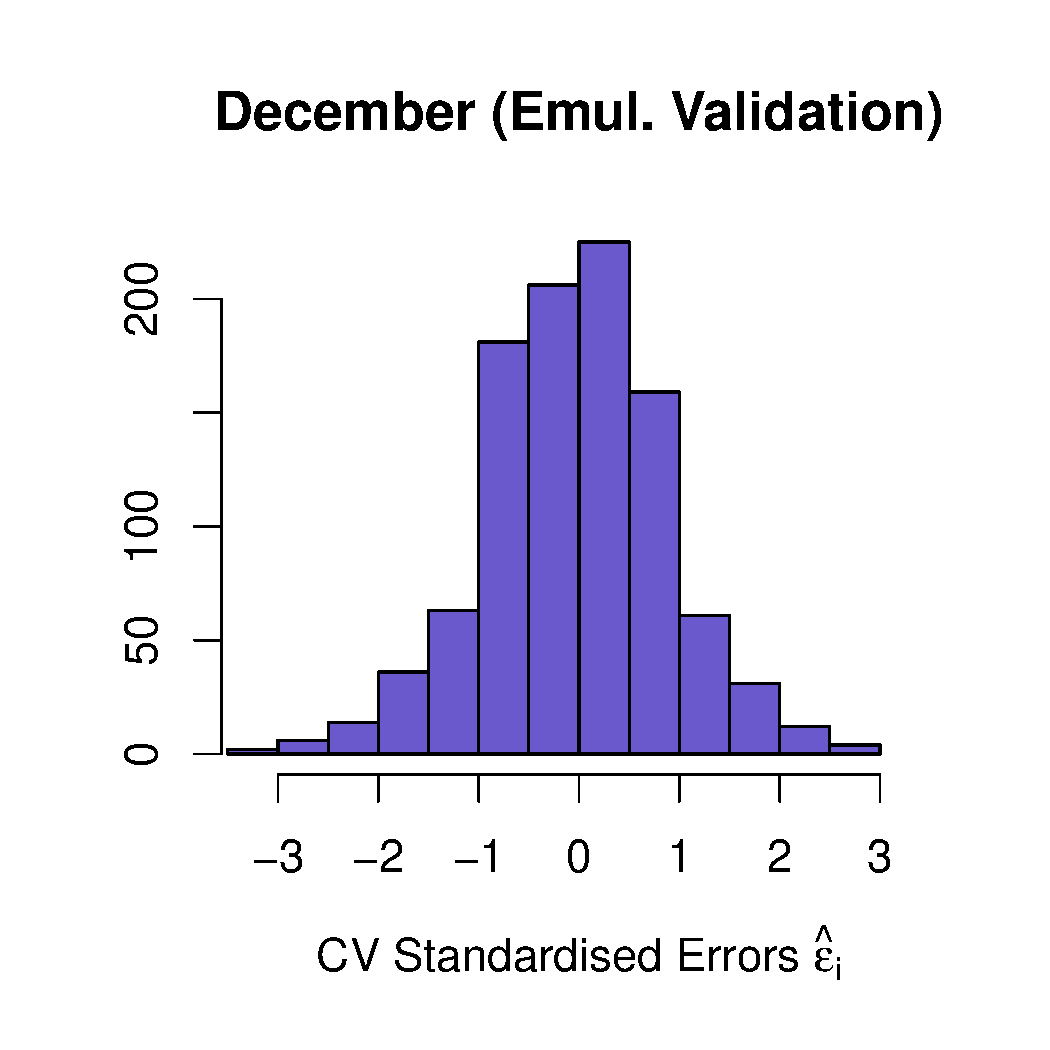
\includegraphics[width=\scale]{Emulator_CV/Histograms/December_CV_Errors_Hist}
 \caption{Validation of the emulators. In each plot, the histogram of the $n=1000$ cross-validated standardised errors $\widehat \eps_i$ is shown (equation~\eqref{Eqn_St_Err}).}
 \label{Fig_Histograms_Errors}
\end{figure}

\renewcommand{\scale}{12.7em}
\begin{figure}
\centering
 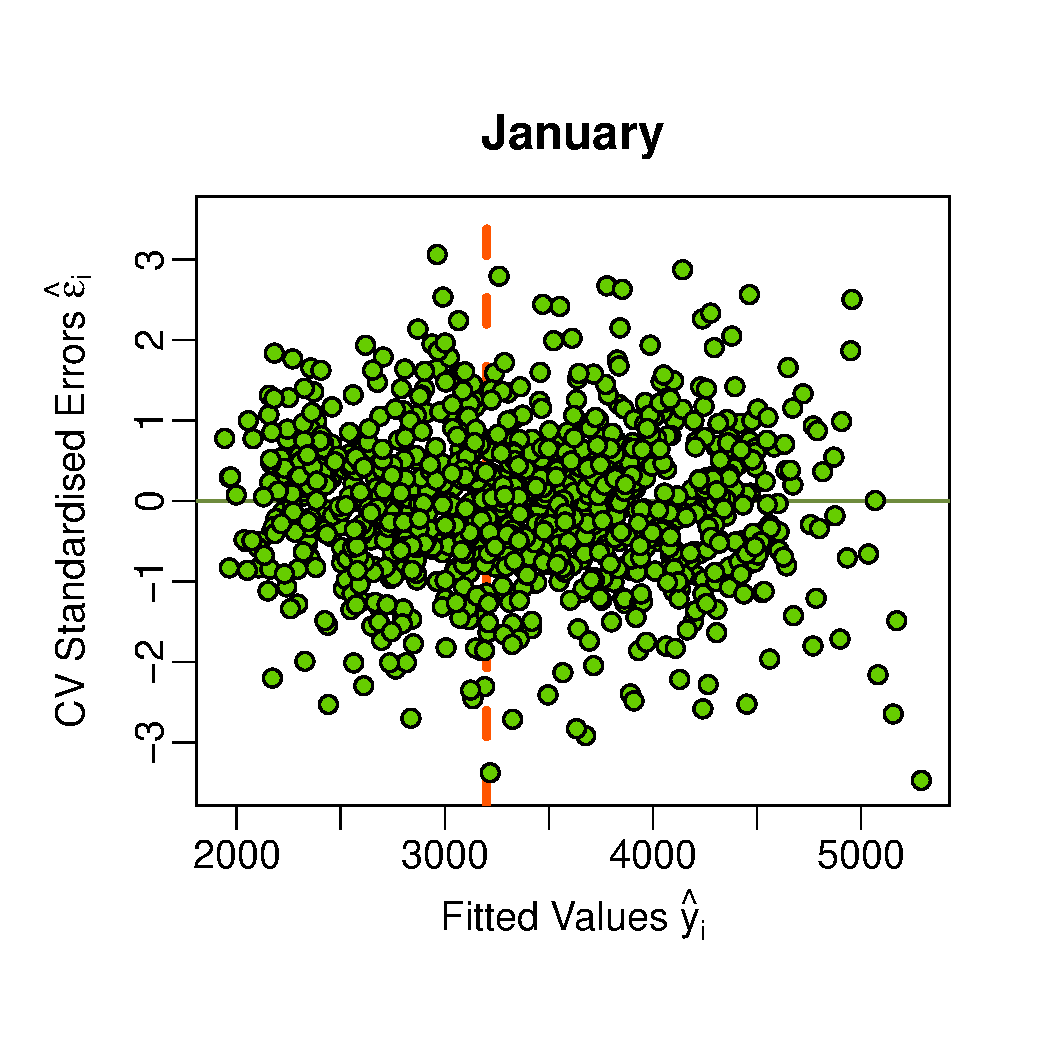
\includegraphics[width=\scale]{Emulator_CV/ScatterPlots/January_CV_Scatter}\hspace{-1ex}
 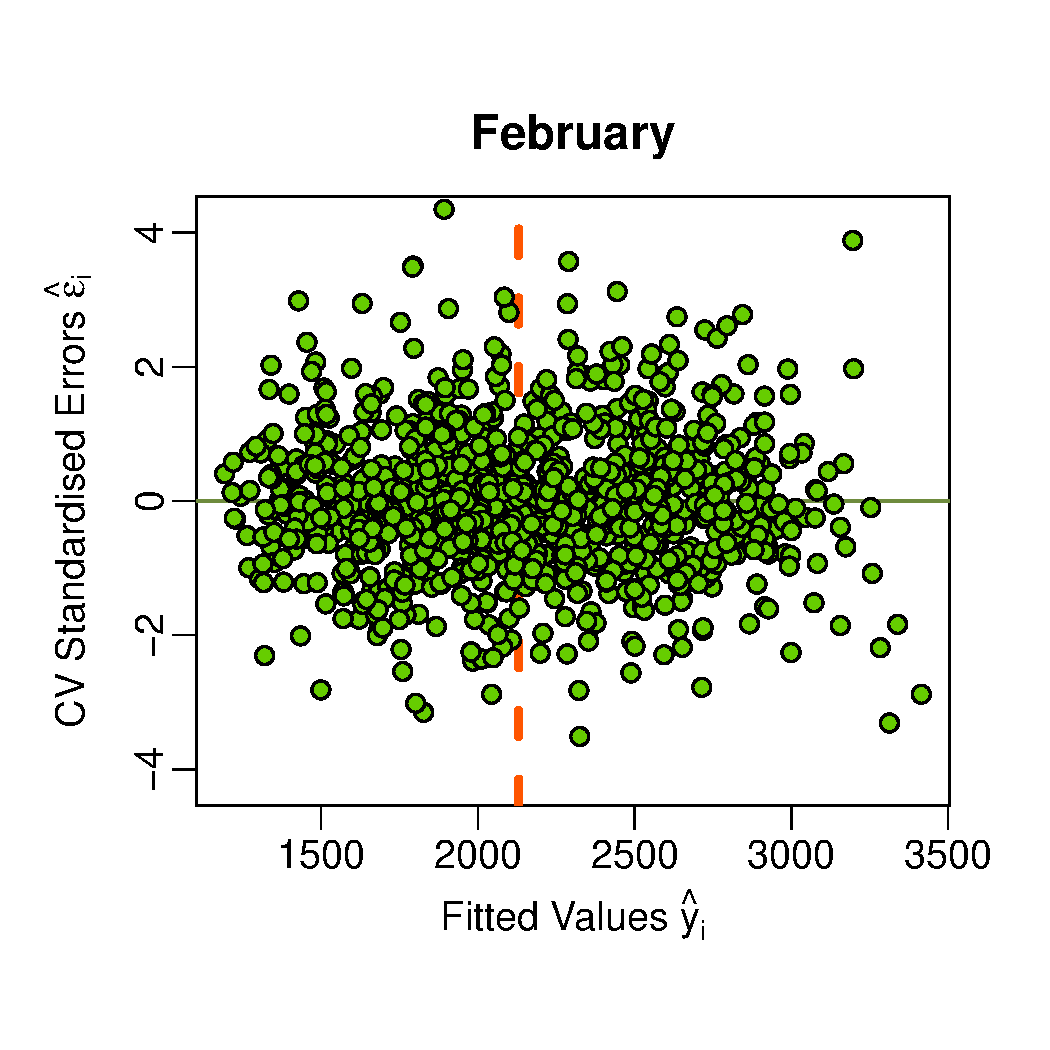
\includegraphics[width=\scale]{Emulator_CV/ScatterPlots/February_CV_Scatter}\hspace{-1ex}
 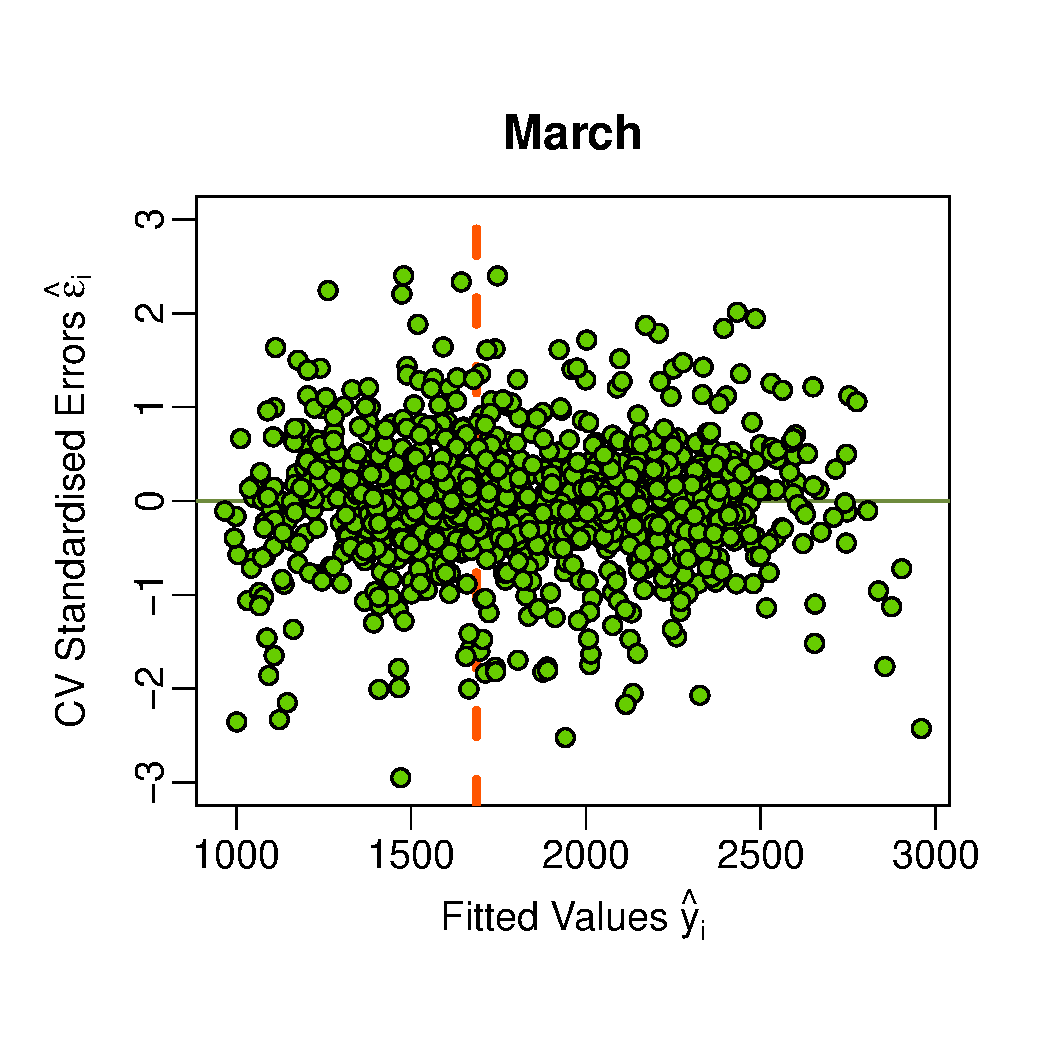
\includegraphics[width=\scale]{Emulator_CV/ScatterPlots/March_CV_Scatter}\\[-3ex]
 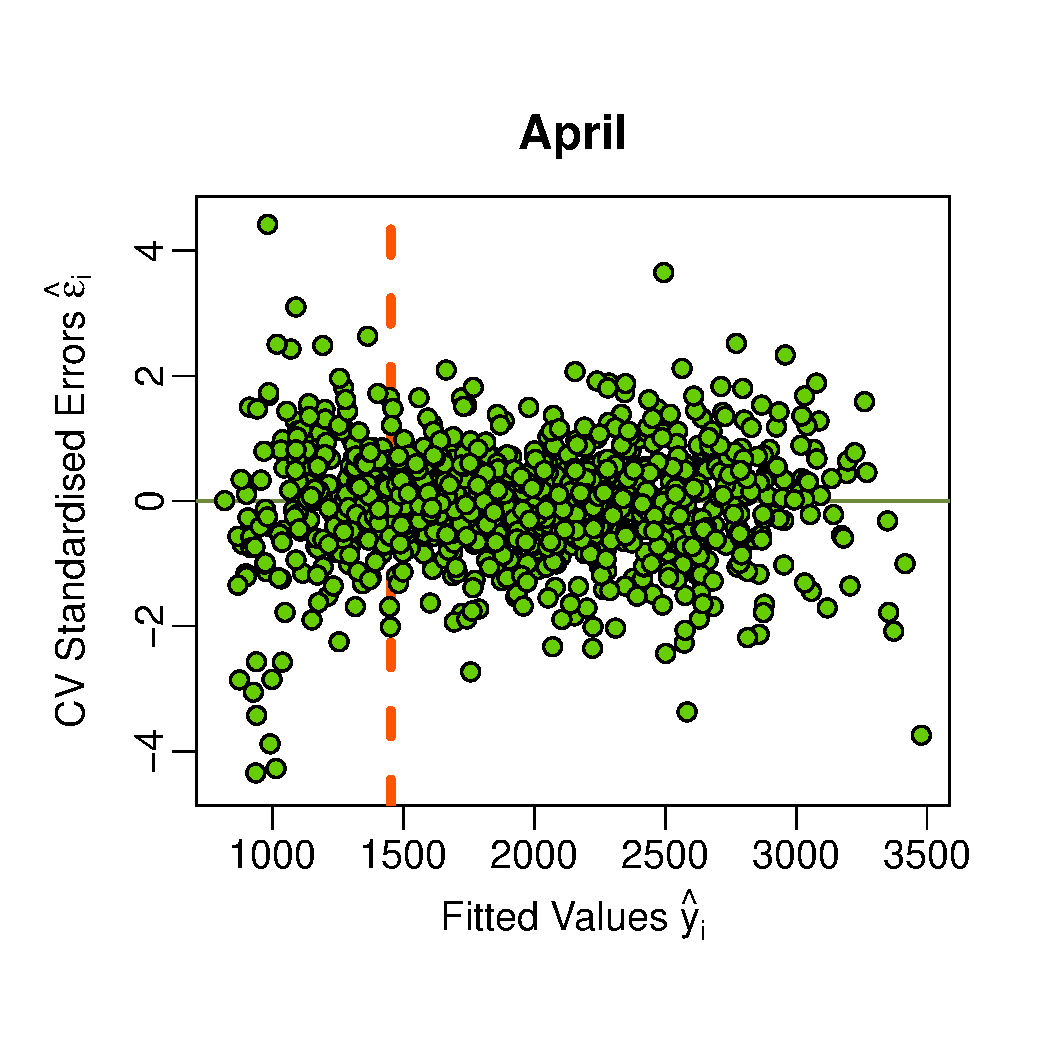
\includegraphics[width=\scale]{Emulator_CV/ScatterPlots/April_CV_Scatter}\hspace{-1ex}
 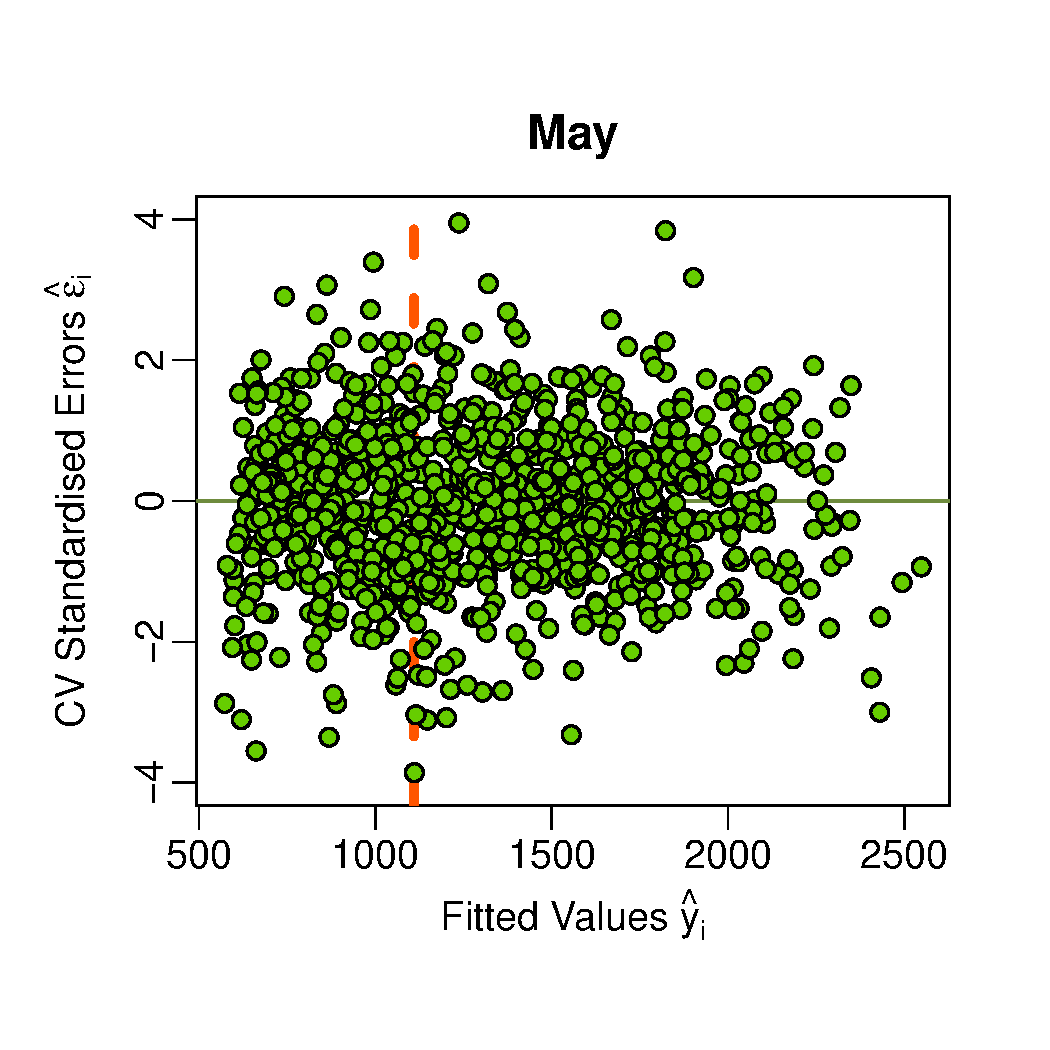
\includegraphics[width=\scale]{Emulator_CV/ScatterPlots/May_CV_Scatter}\hspace{-1ex}
 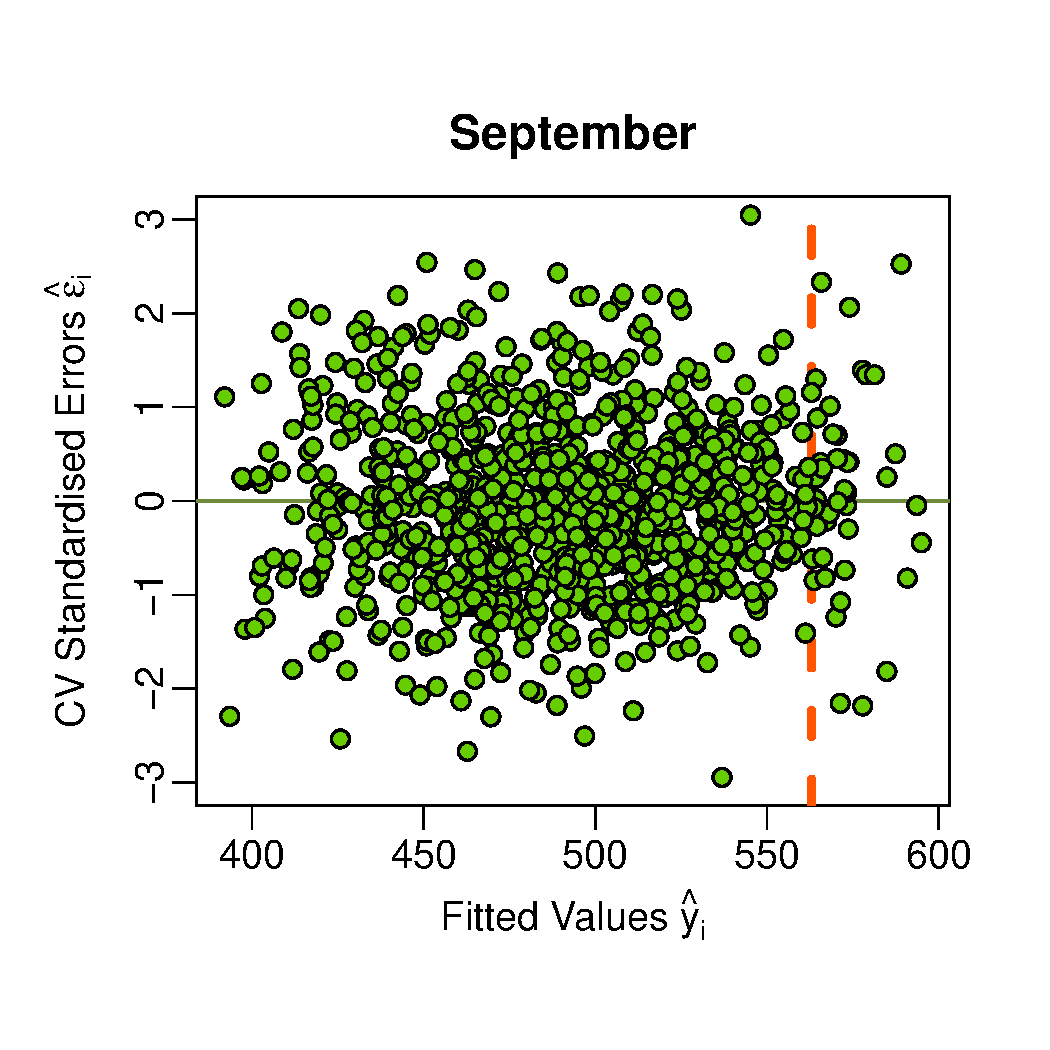
\includegraphics[width=\scale]{Emulator_CV/ScatterPlots/September_CV_Scatter}\\[-3ex]
 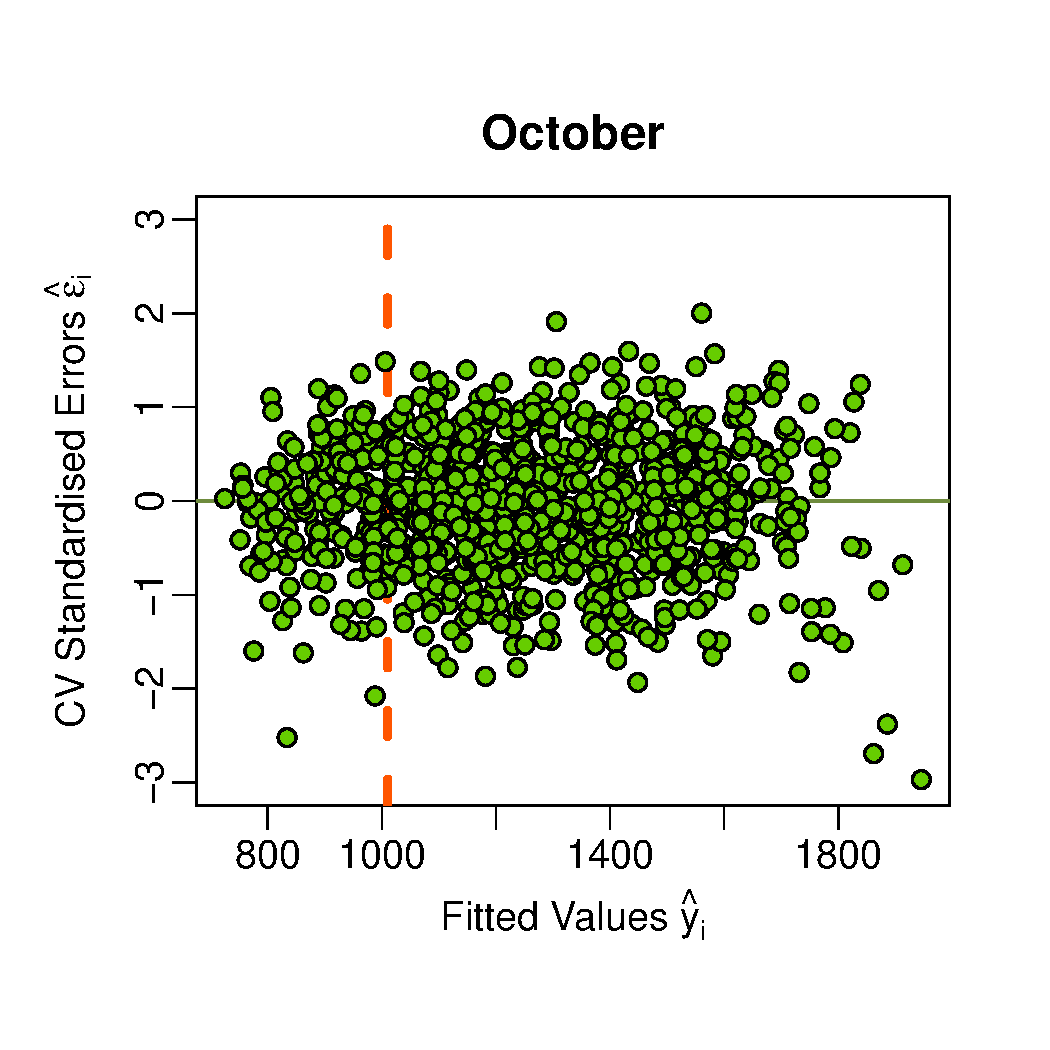
\includegraphics[width=\scale]{Emulator_CV/ScatterPlots/October_CV_Scatter}\hspace{-1ex}
 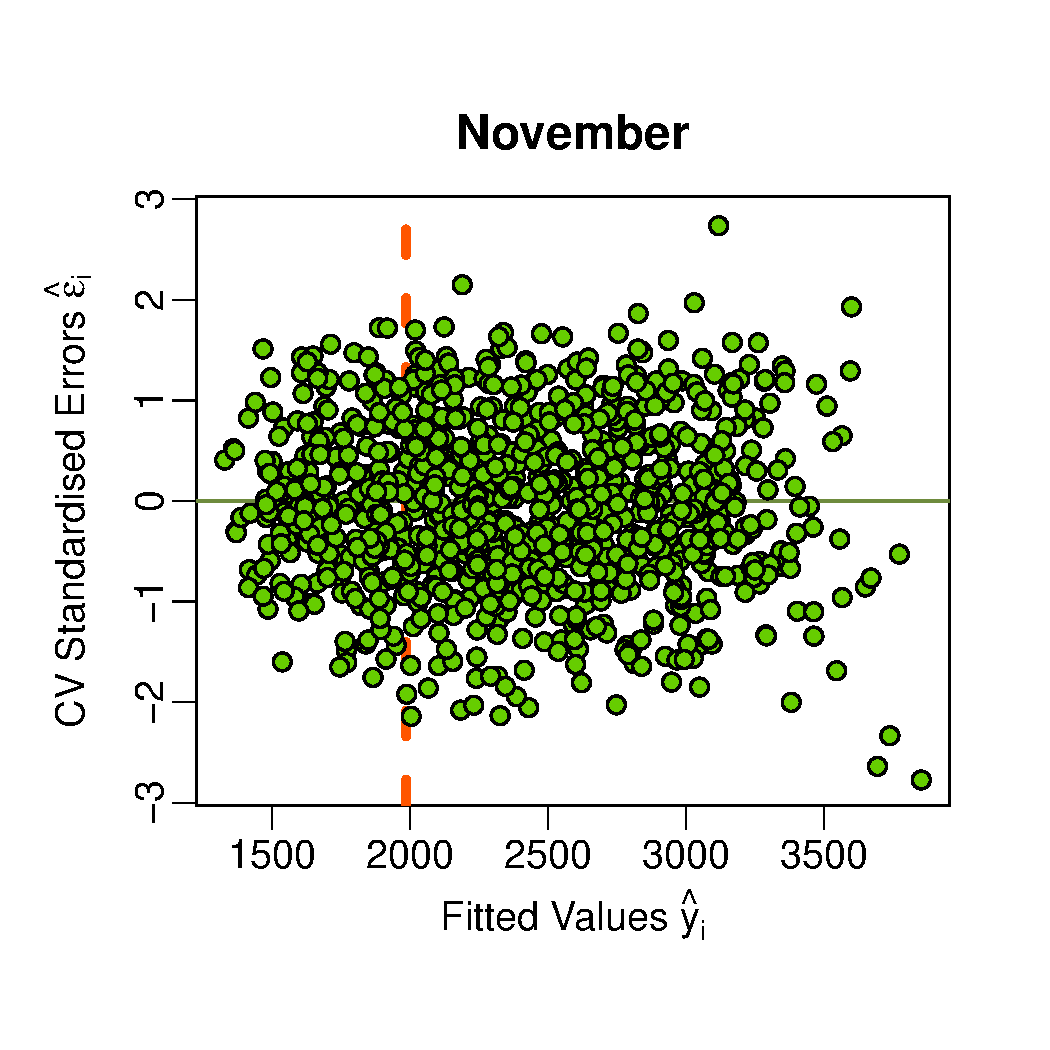
\includegraphics[width=\scale]{Emulator_CV/ScatterPlots/November_CV_Scatter}\hspace{-1ex}
 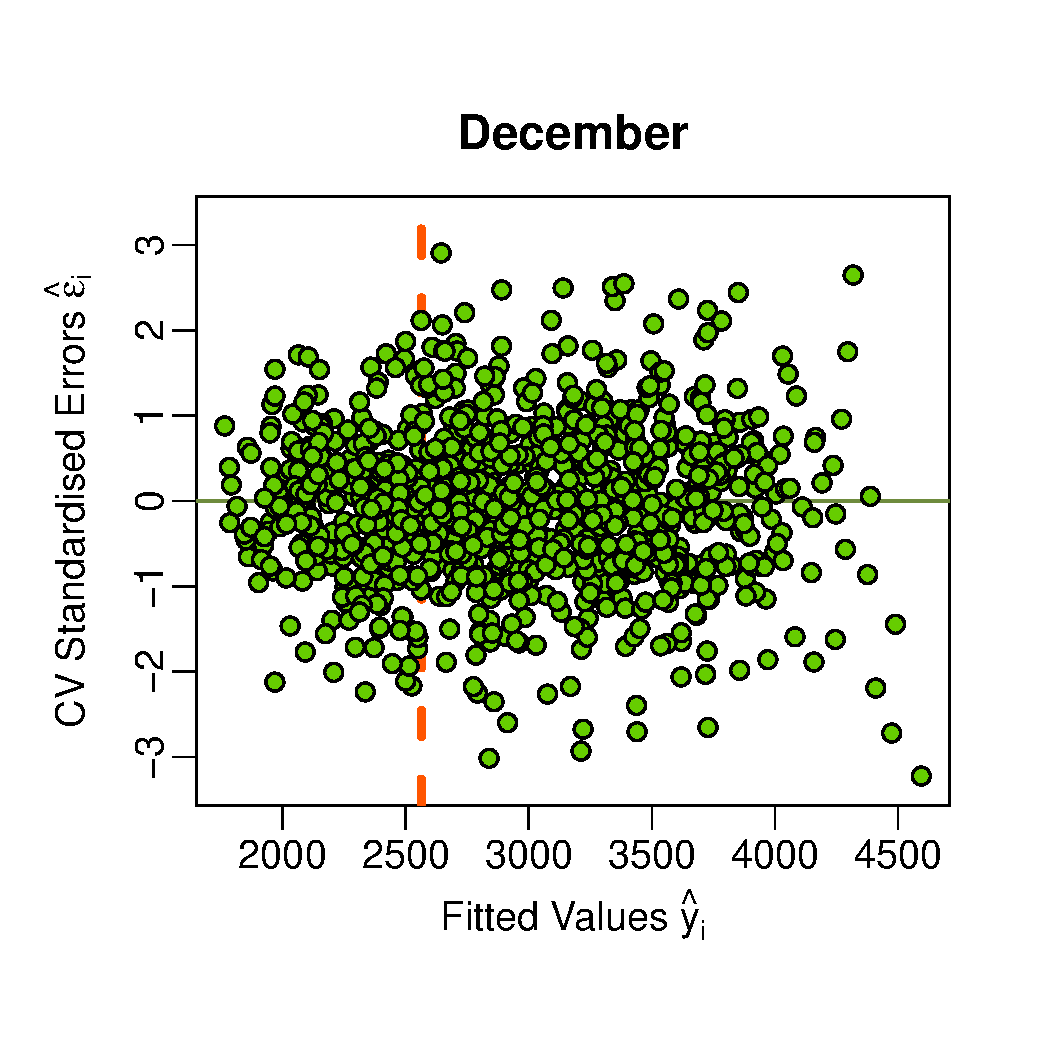
\includegraphics[width=\scale]{Emulator_CV/ScatterPlots/December_CV_Scatter}
 \caption{Validation of the emulators. For the different months, the standardised errors in \eqref{Eqn_St_Err} are plotted against the emulator's fitted values. In each plot, the vertical dashed line identifies the $x$-value at which observed gas consumption for the month is available.}
 \label{Fig_Scatter_Errors}
\end{figure}
\newpage

\section{History Matching}

The emulators built in Section~\ref{Sec_Emulators} allow to predict, for any input $\x \in \R^8$, the simulated gas consumption $f(\x)$ associated with that set of inputs.
Since observed gas consumptions are available for each month, we can use the emulators to select inputs $\x$ whose simulated gas consumptions are ``compatible'' with the observed data.
The context and notation to carry out the comparison are introduced below. 


\subsection{Notation and Choices}
As in the rest of this work, $f(\x)$ will denote the simulated gas consumption associated with input $\x$. With a slight abuse of notation which should however cause no confusion, we denote by $\E[f(\x)]$ and $\Var[f(\x)]$ the emulator mean prediction and variance associated with input $\x$. Finally, we denote by $z \in \R$ the observed gas consumption. Note that, albeit not explicitly signalled in the notation, all these quantities depend on the particular month considered.


When using the emulator to assess the compatibility between the (unknown) value $f(\x)$ corresponding to a given input $\x$, and the available observed consumption $z$, we need to account for at least three different types of uncertainties.
\begin{enumerate}
 \item The emulator prediction is only an approximation to the actual model response
       $f(\x)$: this uncertainty is naturally quantified by the emulator standard deviation associated with the prediction.
 \item Even if the emulator were a perfect reproduction of the simulator, the latter
       would only be an imperfect reproduction of reality. We ultimately want to learn about the real world, so model discrepancy (MD) should be accounted for.
 \item Due to unavoidable measurement errors (MEs), the observed consumption $z$
       differs from the actual amount of gas consumed in the building during the month.
\end{enumerate}

The aim of the first wave of emulators is to discard those inputs $\x$ which, once the previous uncertainties are accounted for, are extremely unlikely to generate an actual consumption $z$ in the real world. In order to quantify the mismatch between an input $\x \in \R^8$ and the observed $z$ for the month $M$, we consider the following implausibility measure\footnote{
I don't add much here, but clearly in a paper we would reference Michael's work and possibly restructure the exposition.}:
\begin{equation}
 I_M(\x) = \frac{\big|\, \E[f(\x)] - z \,\big| }{ \sqrt{
 {\Var[f(\x)]}^{\phantom{i}} \!+ \Var[\epsilon_{_\text{MD}}(\x)] + \Var[\epsilon_{_\text{ME}}(z)] \,}^{\,}
       } \,, \;\quad \x \in \R^8.
\end{equation}
The subscript $M$ denotes the dependence on the month considered (it is omitted from the terms on the right-hand side for simplicity of notation).
The quantity $I(\x)$ is dimensionless. The last two terms of the denominator represent the uncertainty ascribed to model discrepancy and measurement errors respectively, and have the same dimension as $\Var[f(\x)]$.


In our case, we assess the measurement error to be of the order of $5\%$ of the reported gas consumption $z$. To translate this into a value for $\Var[\epsilon_{_\text{ME}}]$, we
make the simplifying assumption that the actual consumption has uniform probability of being anywhere in the interval $[0.975 z, 1.025 z]$. Since the variance of a uniform random variable on an interval of length $L$ is $L^2/12$, the assumption yields:
\begin{equation}
 \Var[\epsilon_{_\text{ME}}(z)] = \frac{z^2}{\,4800\,}\,.
\end{equation}

As far as model discrepancy is concerned, we consider three different scenarios, where the discrepancy between a simulated output $y$ and reality is estimated in about $5\%$, $10\%$ and $20\%$ of $y$ respectively. Since the output $y$ is not available for a general input $\x$, we consider the quantity $\E[f(\x)]$ as its surrogate, therefore computing $\Var[\epsilon_{_\text{MD}}(\x)]$
as
\begin{equation}
\frac{ \,{\E[f(\x)]}^2\, }{4800}\,, \;
\frac{ \,{\E[f(\x)]}^2\, }{1200}\,, \;
\frac{ \,{\E[f(\x)]}^2\, }{300}
\end{equation}
in the three scenarios respectively.



For the month $M$, we define an input $\x$ as ``non-implausible for $M$'' if the value $I_M(\x)$ is lower than a given threshold $T$. Hence, it is natural to define an input as ``non-implausible'' if the previous condition holds true for all the months. That is, if
\begin{equation}\label{Condition}
\max_{M \in \mathcal{M}} \big\{ I_M(\x) \big\} < T\,,
\end{equation}
where $\mathcal{M}$ is the set of nine months considered in this work. Since the previous equation represents the simultaneous imposition of nine conditions, we consider two relatively conservative values of $T$ in equation~\eqref{Condition}: $T=4$ and $T=5$. 

\subsection{Results}
In order to explore the compatibility between different regions of the space and the observed data, we generate a quasi-random sample of $N = 6 \times 10^7$ points in the 8-dimensional cube $C={[-1,1]}^8$ (all inputs have been rescaled onto the range $[-1,1]$ prior to the analysis, see Section~\ref{Sec_Choices}). The sample is generated via a Sobol sequence.


We start by examining the results when $T=4$.
In the case where only $5\%$ model discrepancy (MD) is considered, none of the 60 million points is classified as non-implausible according to condition~\eqref{Condition}. Further inspection also reveals that no point can be found which matches any eight of the nine months simultaneously.
However, by accounting for larger model discrepancy, non-implausible inputs can be found: they constitute $0.33\%$ of the space when $10\%$ MD is accounted for, and $19.5\%$ of the space when MD is increased to $20\%$.


\begin{table}
 \centering
 \renewcommand{\arraystretch}{1.6}
 \setlength{\tabcolsep}{0.9ex}
 \caption{Percentages of non-implausible space when accounting for different size 
          of model discrepancy (MD). Results shown for two different values of the threshold $T$. In the ``All'' column, condition~\eqref{Condition} is used to classify a point as non-implausible.
          The looser condition $I_\text{M}(\x)<T$ is instead used in each of the remaining nine columns, for the different months ``M''
          (percentages rounded to the nearest integer). The ``$\approx 0$'' value in the table corresponds to $1.63 \times 10^{-4} \,\%$ of the space.
          }
 \begin{tabular}{c<{\hspace{2ex}} r<{\hspace{2ex}} ccccccccc}
 \specialrule{0.1em}{0em}{0.1em}
      & {\bf All} & {\bf Jan} & {\bf Feb} & {\bf Mar} & {\bf Apr} & {\bf May} & {\bf Sep} & {\bf Oct} & {\bf Nov} & {\bf Dec} \\
 \specialrule{0.05em}{0.1em}{0.1em}
 \specialrule{0.05em}{0em}{0.5em}
 \multirow{3}{*}{$T=4 \;\left\{ \begin{array}{r}
                                  5\% \text{ MD} \\
                                 10\% \text{ MD} \\
                                 20\% \text{ MD} 
                                \end{array}\right. $}    
                             & 0$\;\;$ & 24 & 24 & 21 & 13 & 14 & 27 & 20 & 19 & 23 \\
                             &   0.33  & 38 & 38 & 33 & 21 & 22 & 45 & 32 & 31 & 36 \\
                             & 19.53   & 70 & 69 & 63 & 39 & 42 & 81 & 59 & 57 & 67 \\
 \specialrule{0.05em}{0.5em}{0.5em}
 \multirow{3}{*}{$T=5 \;\left\{ \begin{array}{r}
                                  5\% \text{ MD} \\
                                 10\% \text{ MD} \\
                                 20\% \text{ MD} 
                                \end{array}\right. $}    
                         & $\approx 0$ & 30 & 30 & 26 & 16 & 18 & 35 & 25 & 24 & 28 \\
                         &    3.36     & 27 & 48 & 42 & 26 & 28 & 58 & 39 & 38 & 45 \\
                         &   37.03     & 84 & 81 & 78 & 50 & 54 & 92 & 74 & 72 & 82 \\ 
  \specialrule{0.1em}{0.5em}{0em}
\end{tabular}
 \label{Table_Implausibility}
\end{table}



In~\autoref{Table_Implausibility} we report these percentages, together with the percentages of space which are deemed non-implausible when compatibility with a single month is imposed. The percentages corresponding to the case $T=5$ are also shown. We see that the non-implausible fraction of space corresponding to a $5\%$ MD is essentially zero also in the $T=5$ case. If we accept that observed consumptions come with a measurement error of at most $5\%$, then this suggests that the discrepancy between the simulator and reality is likely to be higher than $5\%$.


As easily foreseeable from the plots of~\autoref{Fig_Output_Hist}, \autoref{Table_Implausibility} reveals that notable parts of the space result non-implausible when compared with the observation of a single month, although the insersection of these parts of the space may be (almost) empty, as in the two $5\%$ MD cases. With the exception of these two rows, however, we can notice the following: the fraction of non-implausible space is about 2 orders of magnitude higher than the product of non-implausible fractions with respect to the single months. This suggests indeed that the nine conditions imposed in equation~\eqref{Condition} are not independent of each other, but rather positively correlated.

\newpage

\section{Summer Predictions for NROY space}
See \autoref{Fig_Summer}. For the three summer months, the figure compares the output distribution (gas consumption) at:
\begin{enumerate}
\item the original 1000 simulations;
\item the ``non-implausible'' inputs selected after one wave of history-matching.
\end{enumerate}
 




\renewcommand{\scale}{12.2em}
\begin{figure}
\centering
 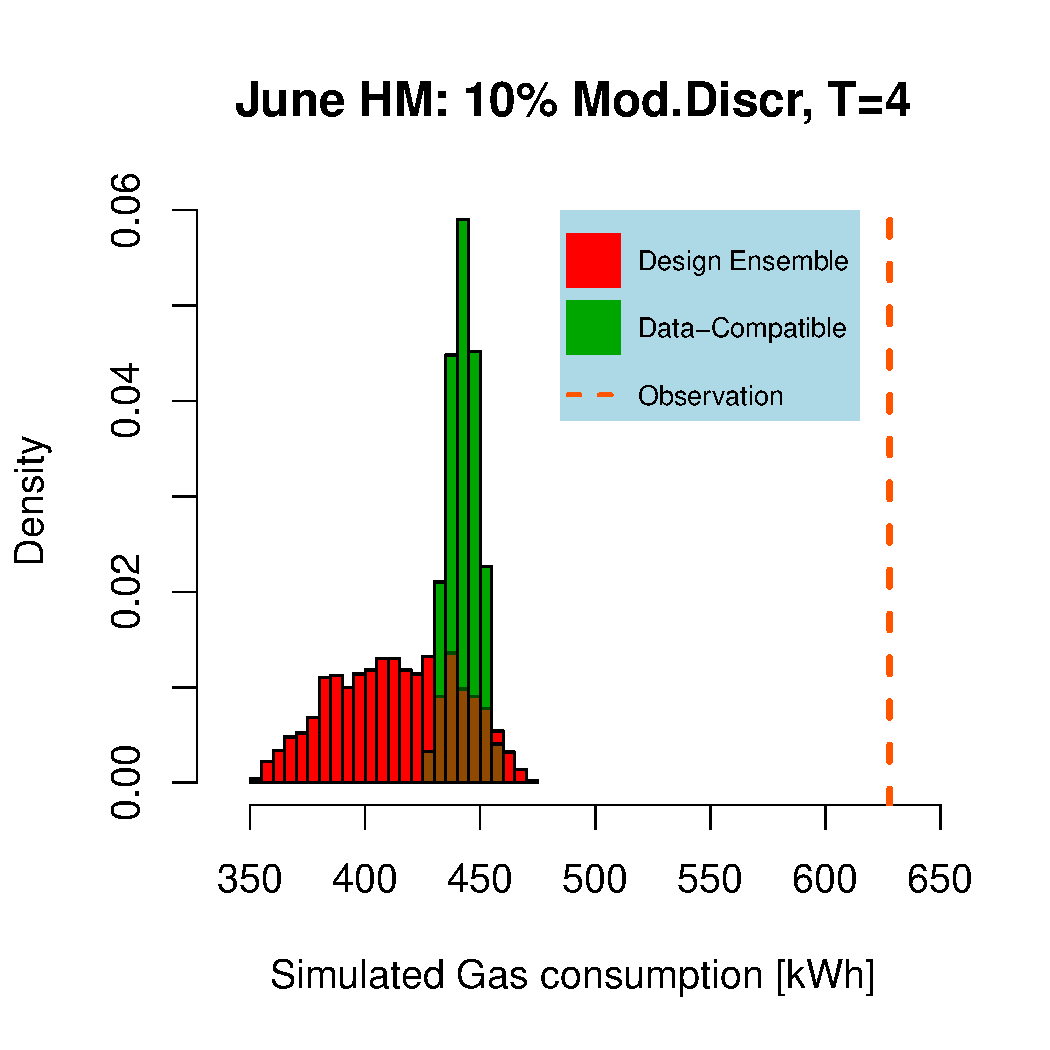
\includegraphics[width=\scale]{Simulation_histograms/HM_Jun-Aug/June_HM_10MD}
 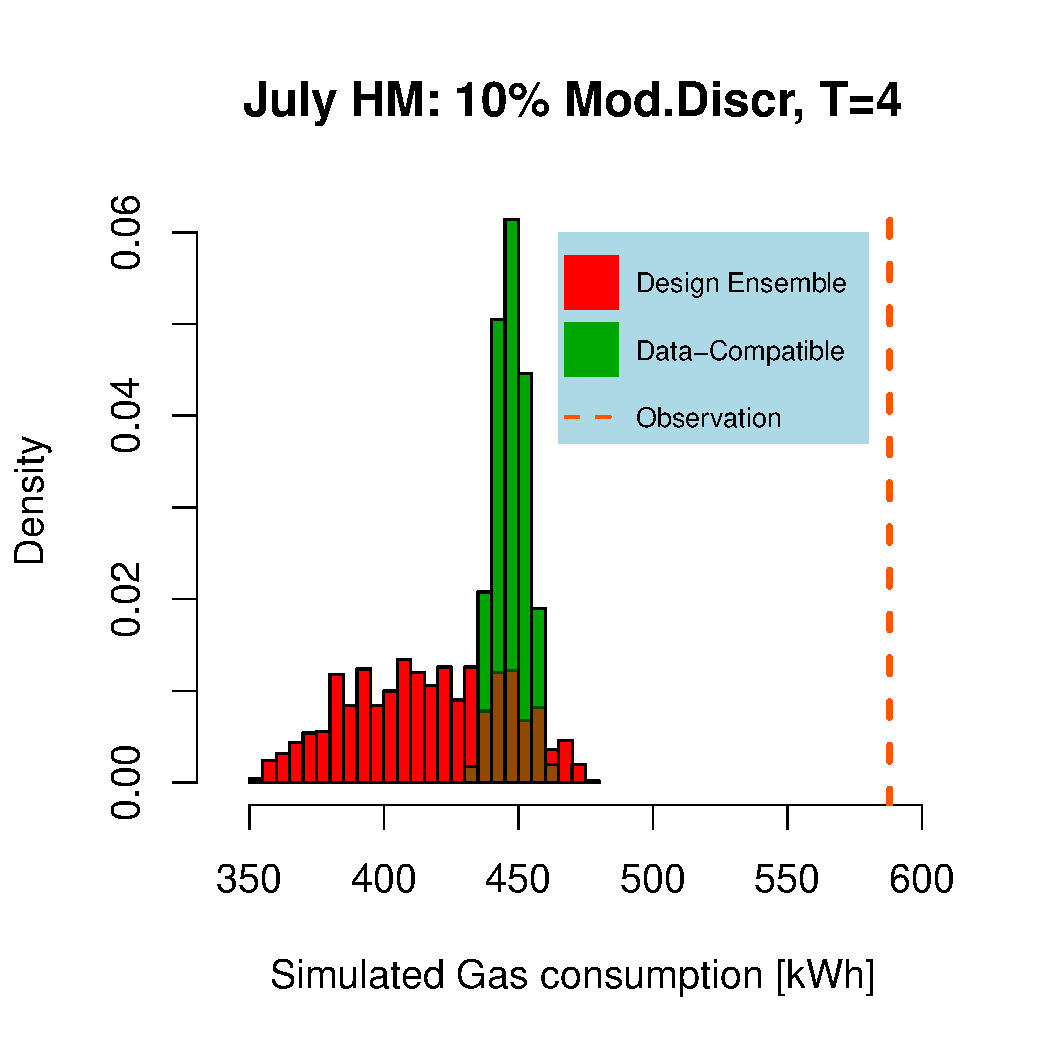
\includegraphics[width=\scale]{Simulation_histograms/HM_Jun-Aug/July_HM_10MD}
 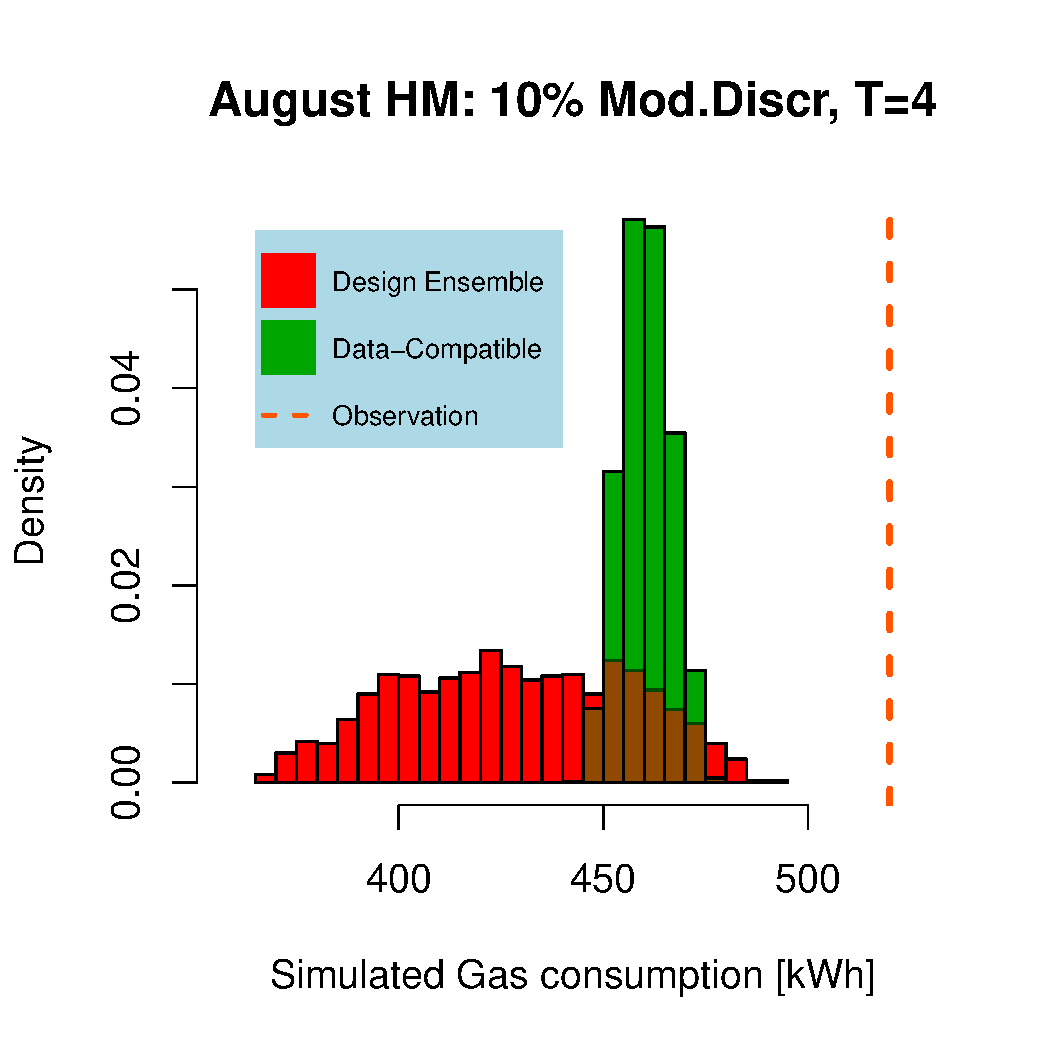
\includegraphics[width=\scale]{Simulation_histograms/HM_Jun-Aug/August_HM_10MD}\\
 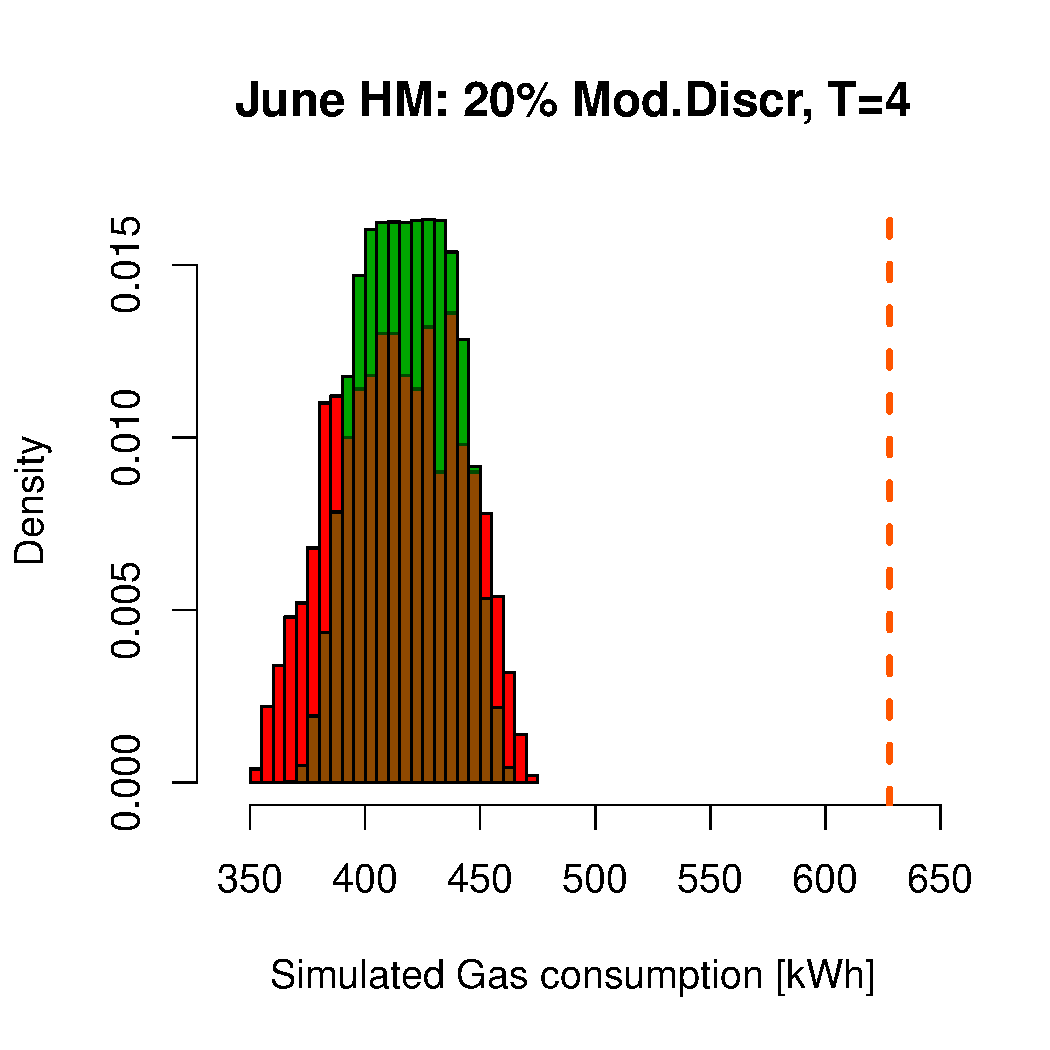
\includegraphics[width=\scale]{Simulation_histograms/HM_Jun-Aug/June_HM_20MD}
 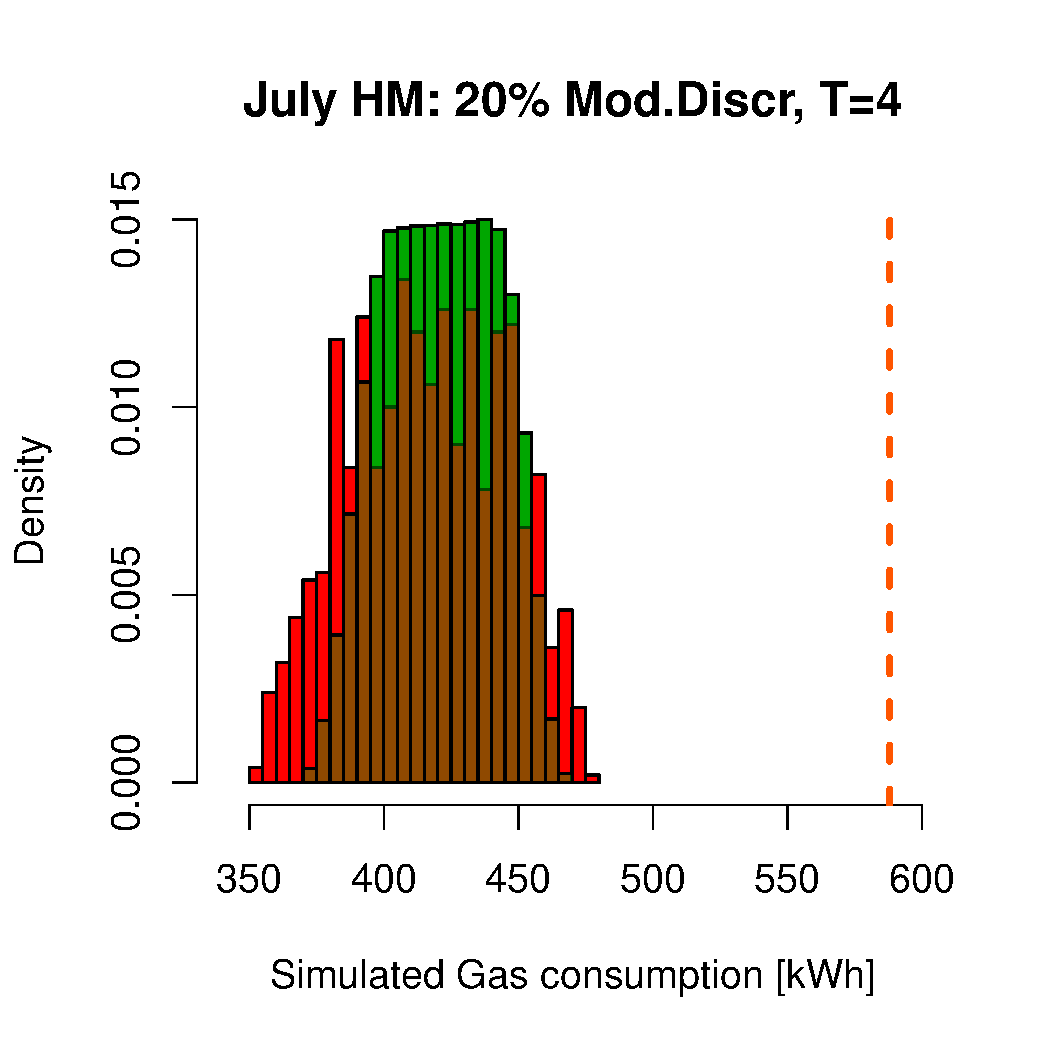
\includegraphics[width=\scale]{Simulation_histograms/HM_Jun-Aug/July_HM_20MD}
 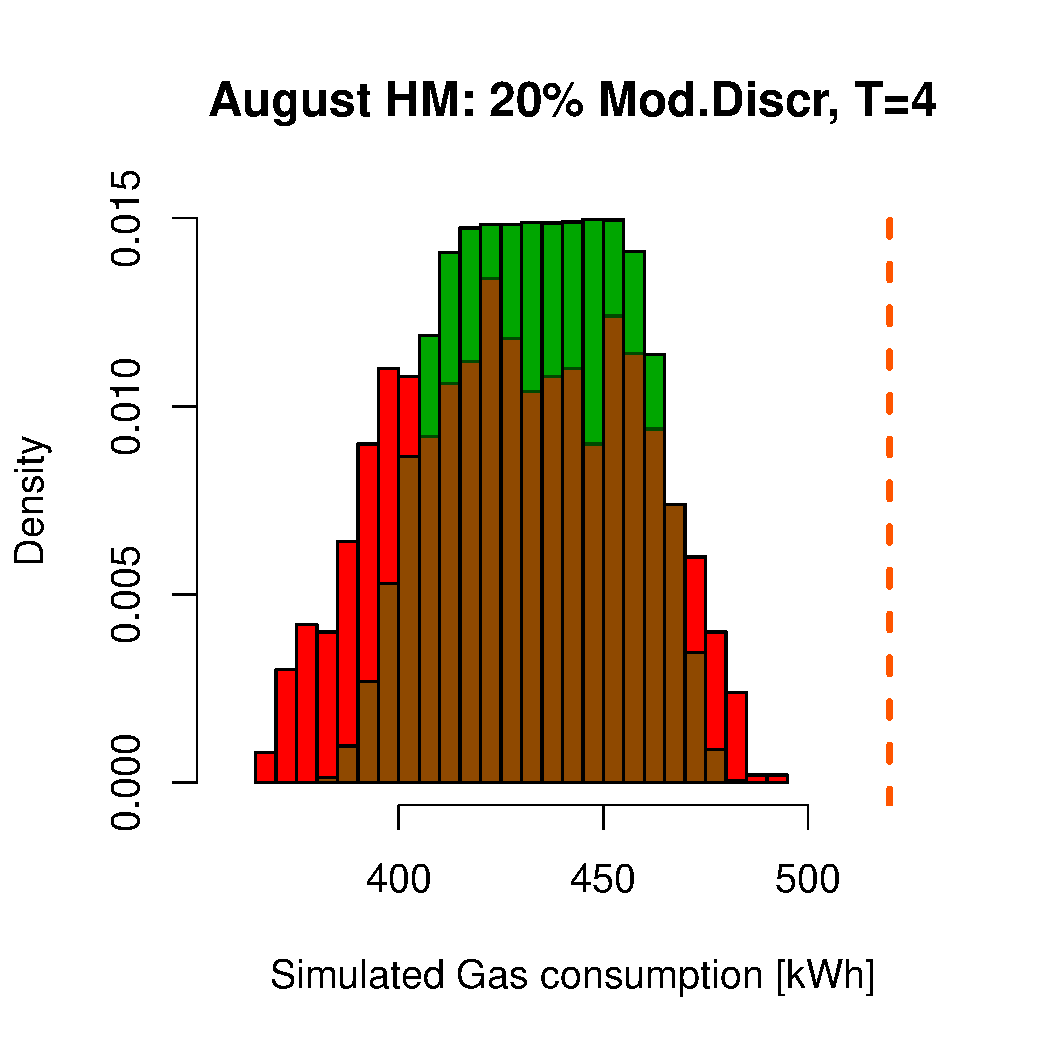
\includegraphics[width=\scale]{Simulation_histograms/HM_Jun-Aug/August_HM_20MD}\\ 
 \caption{Red histograms: distribution of the summer simulated outputs on the $1,000$ design runs (as in \autoref{Fig_Output_Hist}).
 Green histograms: distribution of predicted simulator outputs on NROY inputs after the first wave of simulations.
 The $x$-value of the vertical dashed line in each plot locates the observed consumption for that month.}
 \label{Fig_Summer}
\end{figure}

\newpage

\section{Are some models essentially the same?}

In this section I address the question of whether some of the linear models used to build the emulators of monthly gas consumption (see \autoref{Table_Regressors}) are essentially the same. The question is natural given the very high correlation that the 1000 simulated outputs of some pairs of months show. Specifically, the correlation between the simulated gas consumptions of any two months in the following set
\begin{equation}\label{months}
\{ \text{Jan, Feb, Mar, Apr, Nov, Dec} \}
\end{equation}
is always higher than 0.99, with peaks of more than 0.999 for a few pairs. 

The framework to investigate the question is as follows. Suppose to have two linear models with the same explanatory variables $x_1, \dots, x_n \in \R$
\footnote{The error term is deliberately neglected. Also, notice in our case this is always extremely small, look at the $R^2$ column of \autoref{Table_Regressors}.}:\vspace{-1ex}
\begin{itemize}
\renewcommand\labelitemi{$\blacktriangleright$}
\item M1: $\quad\displaystyle \ya \,=\, \alpha_0 + \sum_{i=1}^n \alpha_i x_i$
\item M2: $\quad\displaystyle \yb \,=\, \beta_0 + \sum_{i=1}^n \beta_i x_i$. 
\end{itemize}
Then, $\ya$ and $\yb$ have correlation one if and only if there exists $b,m \in \R$ such that:
\begin{align}
 \yb &= b + m \ya  \label{corr1}   \\[1ex]
\Longleftrightarrow \qquad \quad
      \beta_0 + \sum_{i=1}^n \beta_i x_i &= b+ m \Big( \alpha_0 + \sum_{i=1}^n \alpha_i x_i \Big) \quad\; \forall \,x_i\nonumber\\
\Longleftrightarrow \qquad 
      \beta_0 - (b+ m \alpha_0) &=  \sum_{i=1}^n (m\alpha_i - \beta_i) x_i \qquad\; \forall \,x_i \nonumber\\[1ex]
\Longleftrightarrow \quad\;\:\,
     \textcolor{RedOrange}{\beta_0 = b+ m \alpha_0} \quad &\text{ and } \quad 
     \textcolor{RedOrange}{\beta_i=m\alpha_i} \quad\forall \,i=1, \dots,n. \label{ya_yb}
\end{align}

The ``$\Rightarrow$'' direction of the last equivalence follows by first taking all $x_i=0$, which yields $\beta_0 = b + m\alpha_0$. Hence, the choice $x_i=1$ and $x_j=0$ for $j\neq i$ yields condition \eqref{ya_yb}.

In words, we have shown that the models M1 and M2 generate responses with correlation one iff there exists $m\in \R$ such that
\begin{equation}
\beta_i=m\alpha_i \qquad \forall\, i=1, \dots,n.
\end{equation}
The ``intercept'' coefficients $\alpha_0$ and $\beta_0$ can instead be anything: the value of $b$ in \eqref{corr1} will be obtained as $b=\beta_0 - m\alpha_0$. 
%In the special case $\beta_0 = m\alpha_0$, the response variables $\ya$ and $\yb$ will just be a multiple of the other.

On the above basis, let's look at pairs of gas consumption linear models, for the six months in \eqref{months}. From \autoref{Table_Regressors}, note indeed that the linear models for these months, each built independently on 1000 observations, all share the same $n=10$ regressors. 

For convenience of notation, if $\bd \alpha=(\alpha_0, \dots, \alpha_n)$ are the $n+1$ coefficients of the linear model for a month, I'll denote by $\ta \in \R^n$ the portion of $\bd \alpha$ concerning the actual $n$ regressors:
$$
\bd \alpha = (\alpha_0, \ta) \in \R^{n+1}, \quad
\ta=(\alpha_1, \dots, \alpha_n) \in \R^n.
$$

Let then $\bd\alpha, \bd\beta \in \R^{n+1}$ ($n=10$) be the regression coefficients associated with any two months in \eqref{months}. To measure the extent to which $\ta = m \tb \in \R^n$ for some $m$, I have run a simple linear regression, \emph{with no intercept term}, of $\tb$ vs $\ta$. This is done for all 15 possible pairs of months in \eqref{months}. 
The $R^2$ of the 15 LRs is always very good, in some cases remarkably high (IQR=$[0.9923, 0.9987]$, min=0.977, max=0.9996).

\autoref{Fig_LR_Jan} shows the scatter plots of $\tb$ against $\ta$, when $\ta$ are the coefficients for January and $\tb$ the coefficients for the other 5 months in \eqref{months}. The line $y = mx$ is added, $m$ given by the least-square estimate found via the above LRs. The fits are indeed very good\footnote{The scatter plot most deviating from a straight line through the origin is the Jan-Apr one, which is also the one whose $R^2$ is lowest among all 15 pairs of months  ($R^2=0.977$)}.
I have also regressed $\tb$ against $\ta$ \emph{by including an intercept term to the model} (\ie~$\tb\sim q + m \ta$): predictably, the intercept estimate $q$ turns out to be highly non-significant in all cases \mbox{($p$-values close to 1).}

\textcolor{red}{\textbf{\underline{Conclusion}}}: The model coefficients $\bd \alpha$ and $\bd \beta$ for the modelled gas consumptions $\ya$ and $\yb$ of any two months in \eqref{months} essentially satisfy $\tb = m\ta$ for appropriate $m\in \R$ (note the tilde). In light of equations (\ref{corr1},\ref{ya_yb}), we can say that $\yb \simeq b + m \ya$, where $b= \beta_0 - m\alpha_0$.




\renewcommand{\scale}{0.443}
\begin{figure}
\centering
 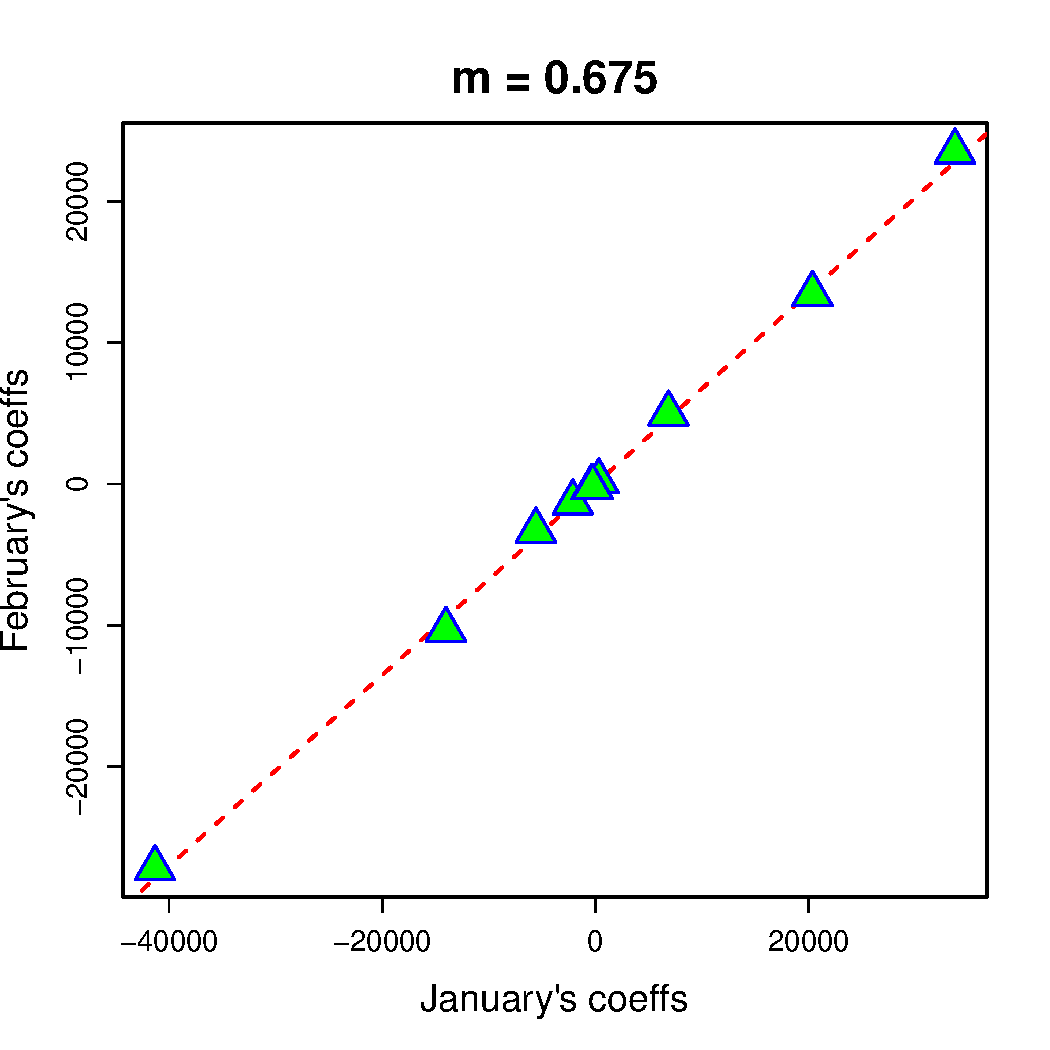
\includegraphics[scale=\scale]{Compare_LRs/LR_Jan_Feb}\hspace{-1ex}
 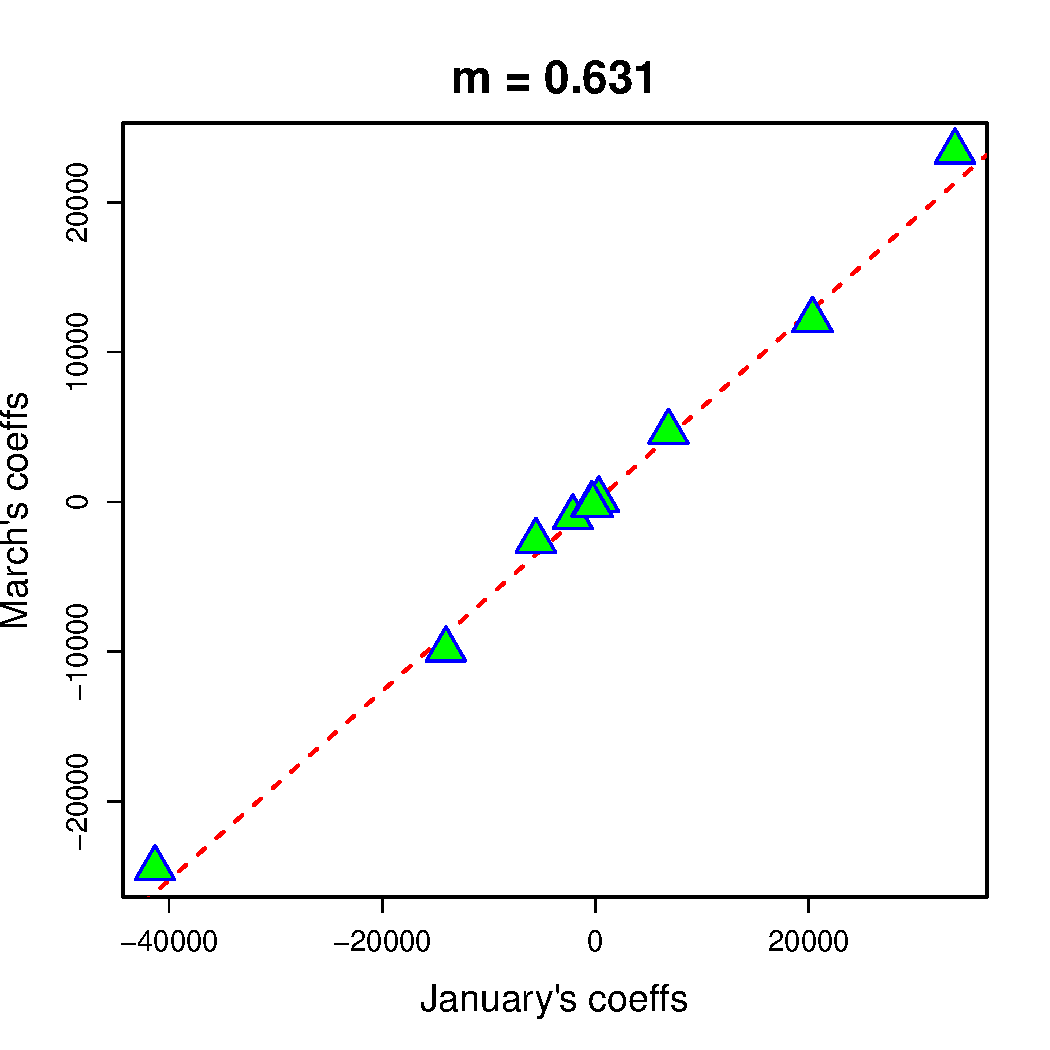
\includegraphics[scale=\scale]{Compare_LRs/LR_Jan_Mar}\hspace{-1ex}
 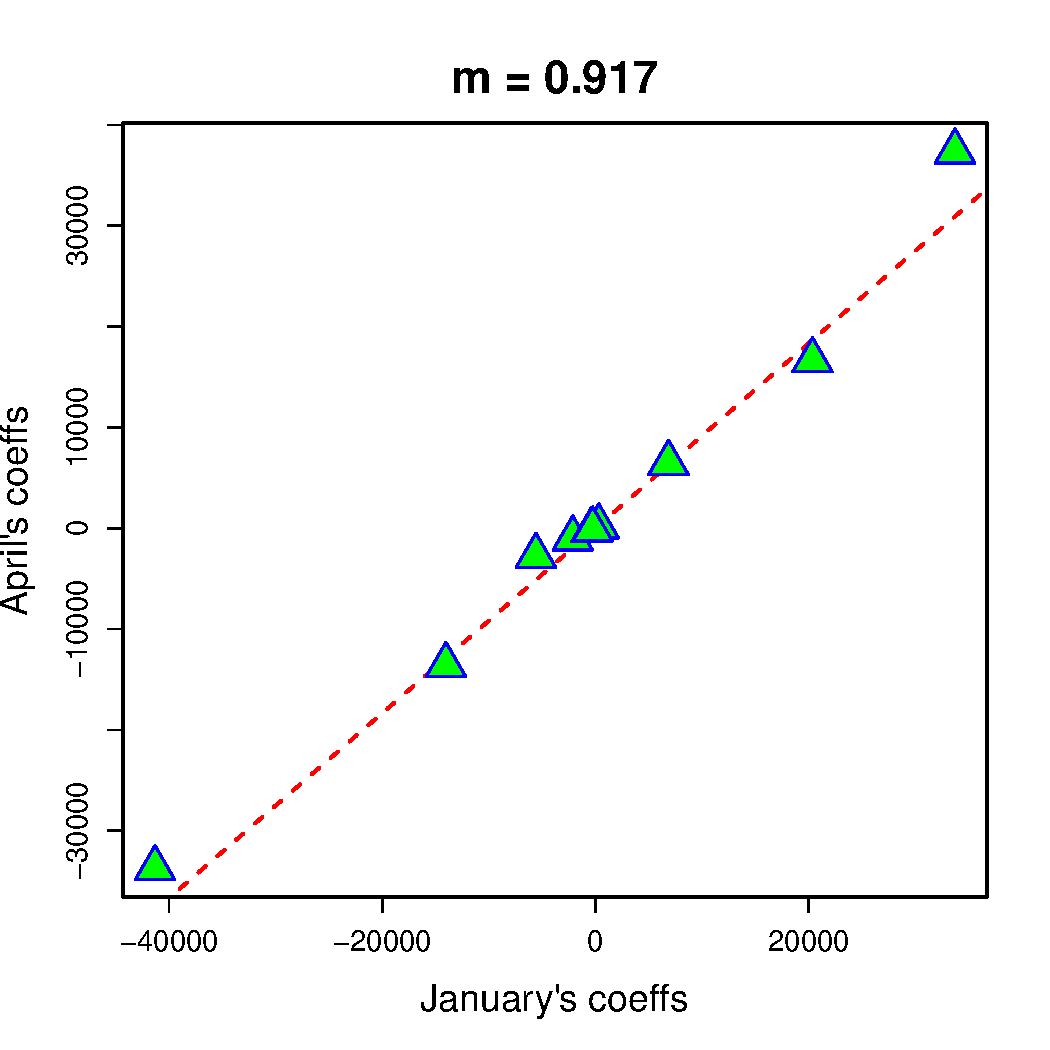
\includegraphics[scale=\scale]{Compare_LRs/LR_Jan_Apr}\hspace{-1ex}
 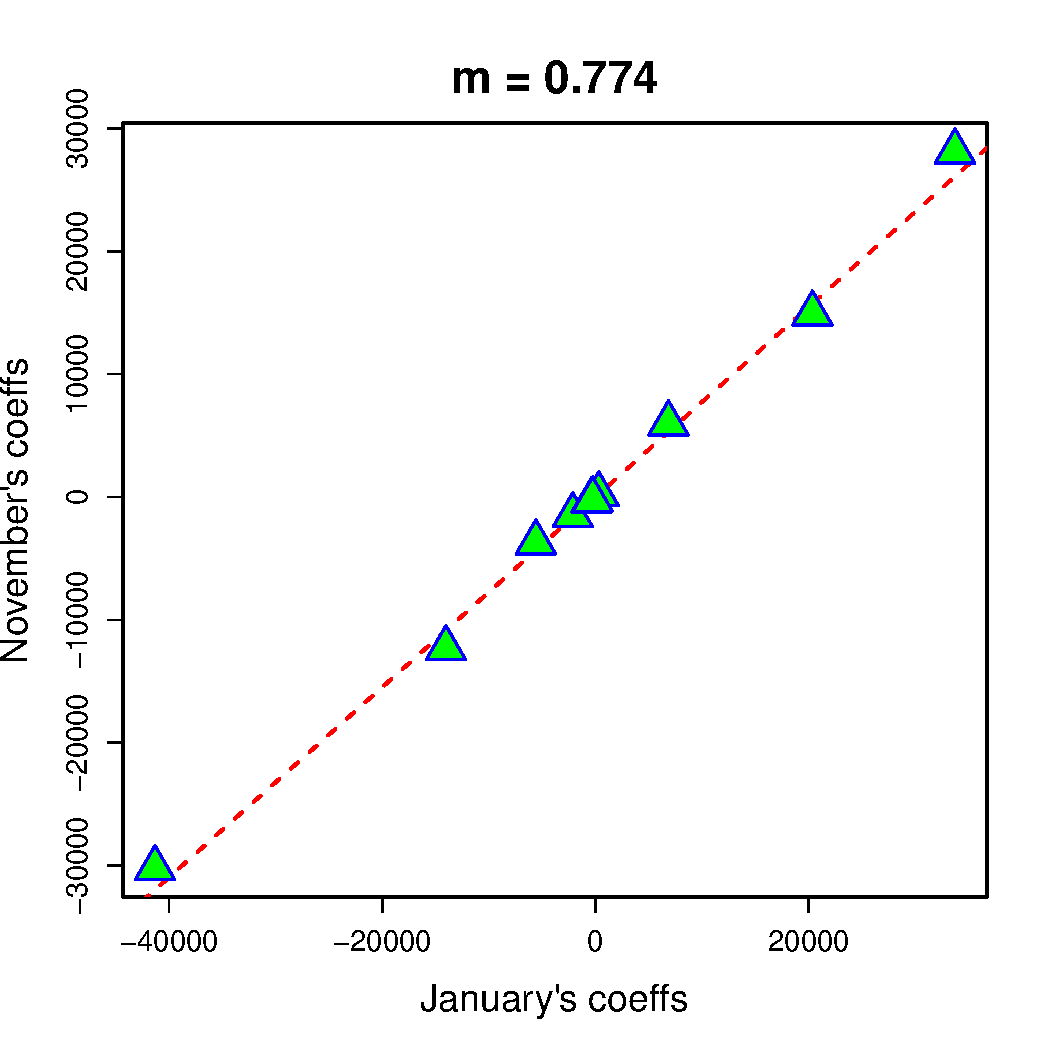
\includegraphics[scale=\scale]{Compare_LRs/LR_Jan_Nov}\hspace{-1ex}
 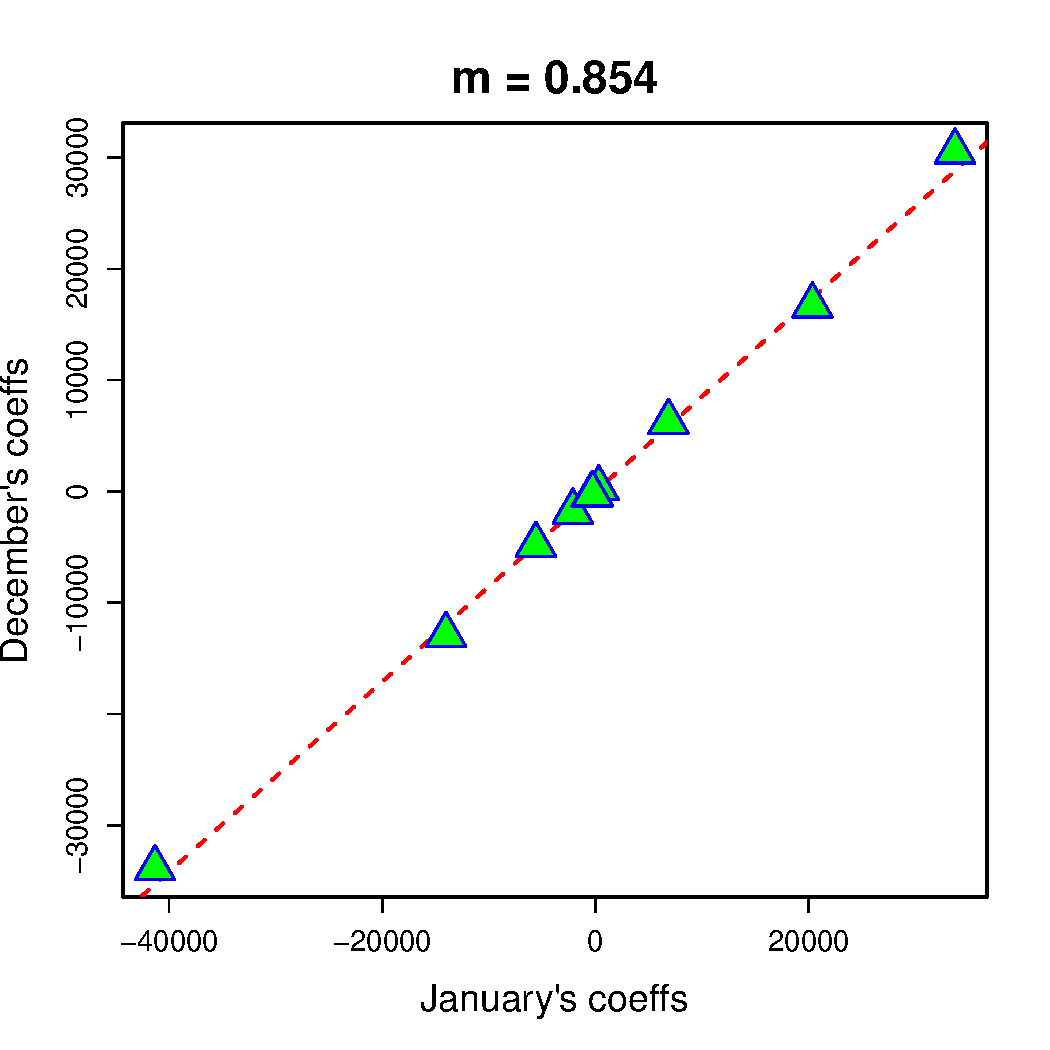
\includegraphics[scale=\scale]{Compare_LRs/LR_Jan_Dec}
 \caption{Scatter plots of the 10 LR coefficients estimated by regressing monthly gas consumption on 10 covariates (see~\autoref{Table_Regressors}). Plots concerning the months in \eqref{months} against January coefficients are reported. An approximate linear relationship of the form $y=mx$ can be observed in all cases. The value of $m$ is estimated by least squares and displayed \mbox{on top of each panel.}}
 \label{Fig_LR_Jan}
\end{figure}


\newpage

\section{Temperature Data}
In addition to energy use predictions, at any configuration $\x \in \R^8$ of the eight inputs (see \autoref{Table_Var_names}) the simulator returns predicted temperature in two rooms of the house: the kitchen and the master room. 
Measurements of observed temperature in the two rooms are also available. 
We would like to use both the energy and the environmental simulated information to reduce the uncertainty on the values on the inputs which lead to a ``reasonable'' match with the corresponding observations.

\subsection{Features of the Time Series}
Observed and simulated temperatures in each of the two rooms come in the form of hourly time series spanning the entire year being simulated (2016). Each time series therefore comprises $8760 = 24 \times 365$ temperature records. 
% The two time series of observed temperatures lack records for the period between Jan, 12$^\text{th}$ and Jan, 21$^\text{st}$.

\begin{figure}
\centering
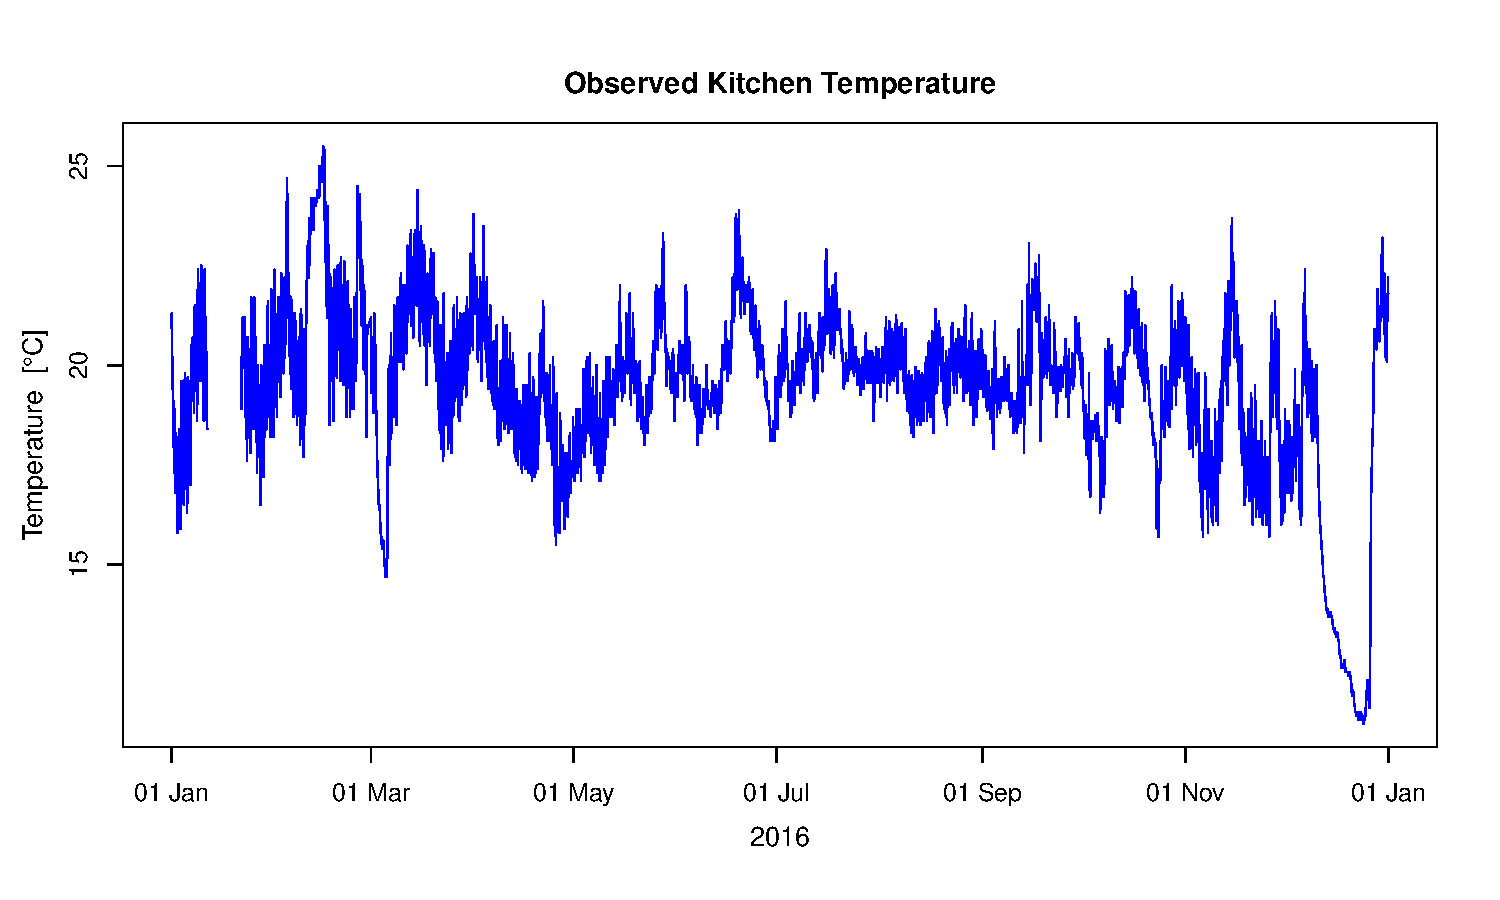
\includegraphics[scale=0.63]{Temperatures/Observed/Obs_Kitch}
\caption{Hourly time series of observed temperature in the kitchen. }
\label{Fig_Obs_Temp}
\end{figure}

\autoref{Fig_Obs_Temp} shows the time series of measured kitchen temperatures\footnote{The time series for the master room that I currently have would be the same and is therefore not shown.}. Records for the period between Jan, 12$^\text{th}$ and Jan, 21$^\text{st}$ are missing.
The drop in recorded temperature between approximately the $10^\text{th}$ and the $26^\text{th}$ of December reflects the lack of occupancy of the building for the period in question. 

%\autoref{Fig_Sim_Temp} shows examples of simulated kitchen temperature time series. The main feature that those plots reveal is the following: during colder months, simulated temperature is not allowed to exceed a given threshold, whose value is characteristic to the simulation.

\newcommand{\scl}{0.38}
\begin{figure}
\centering
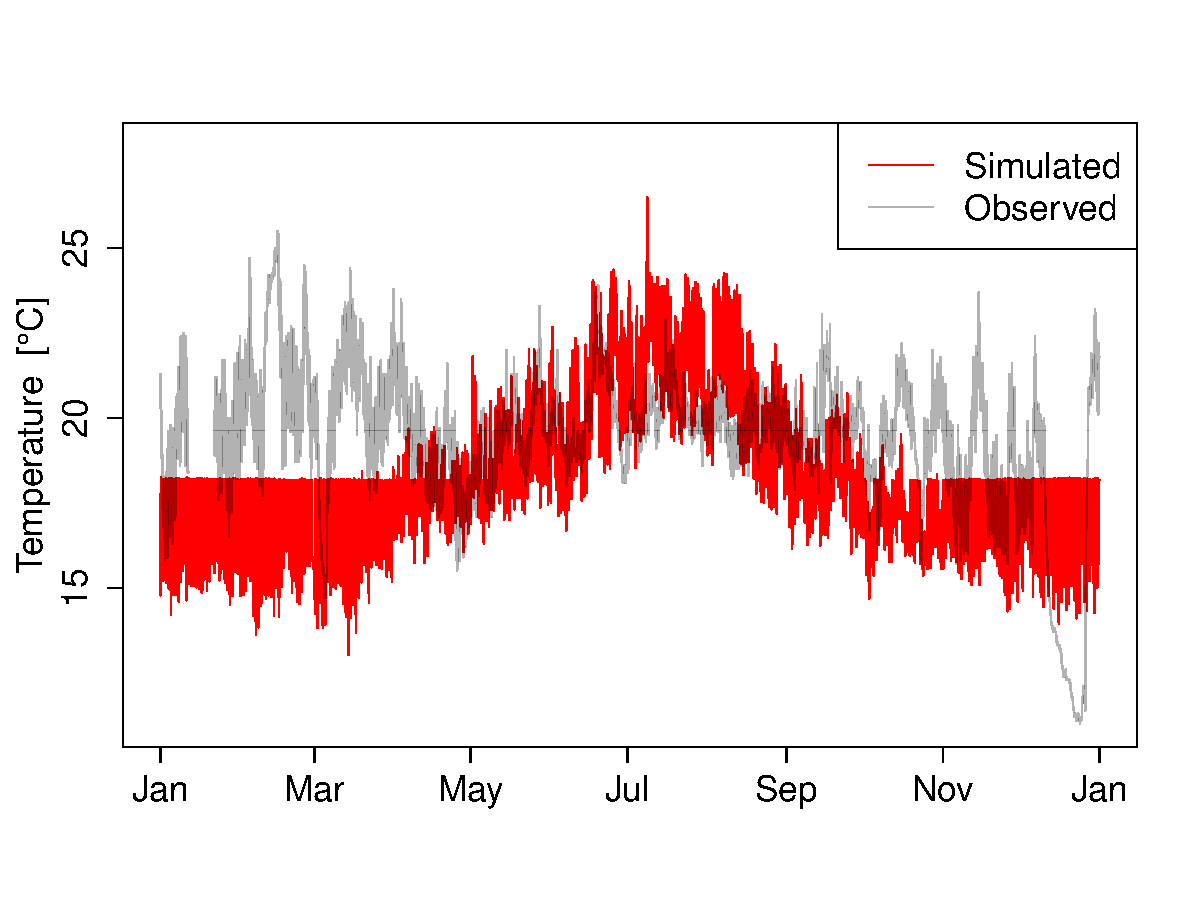
\includegraphics[scale=\scl]{Temperatures/Simulated/Sim_Kitch_863}
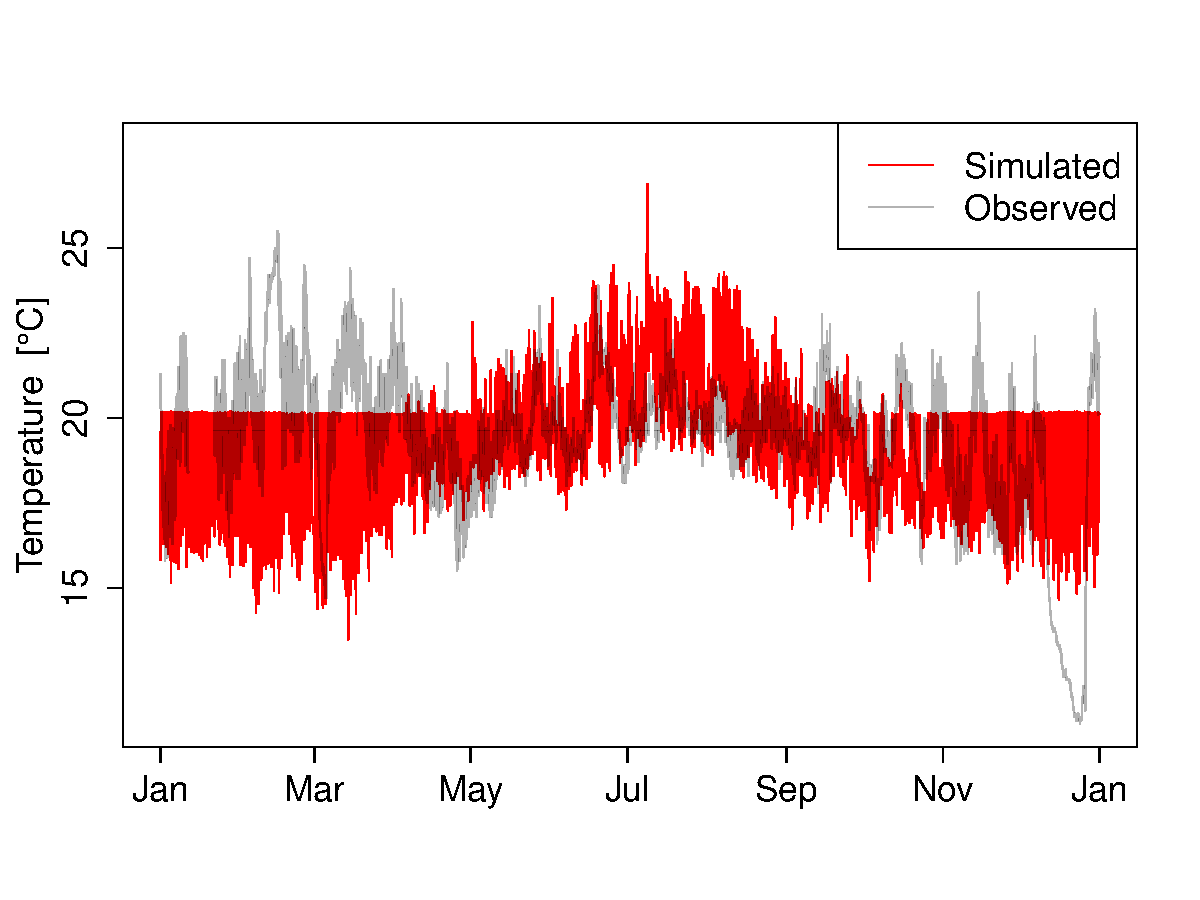
\includegraphics[scale=\scl]{Temperatures/Simulated/Sim_Kitch_384_noylab}
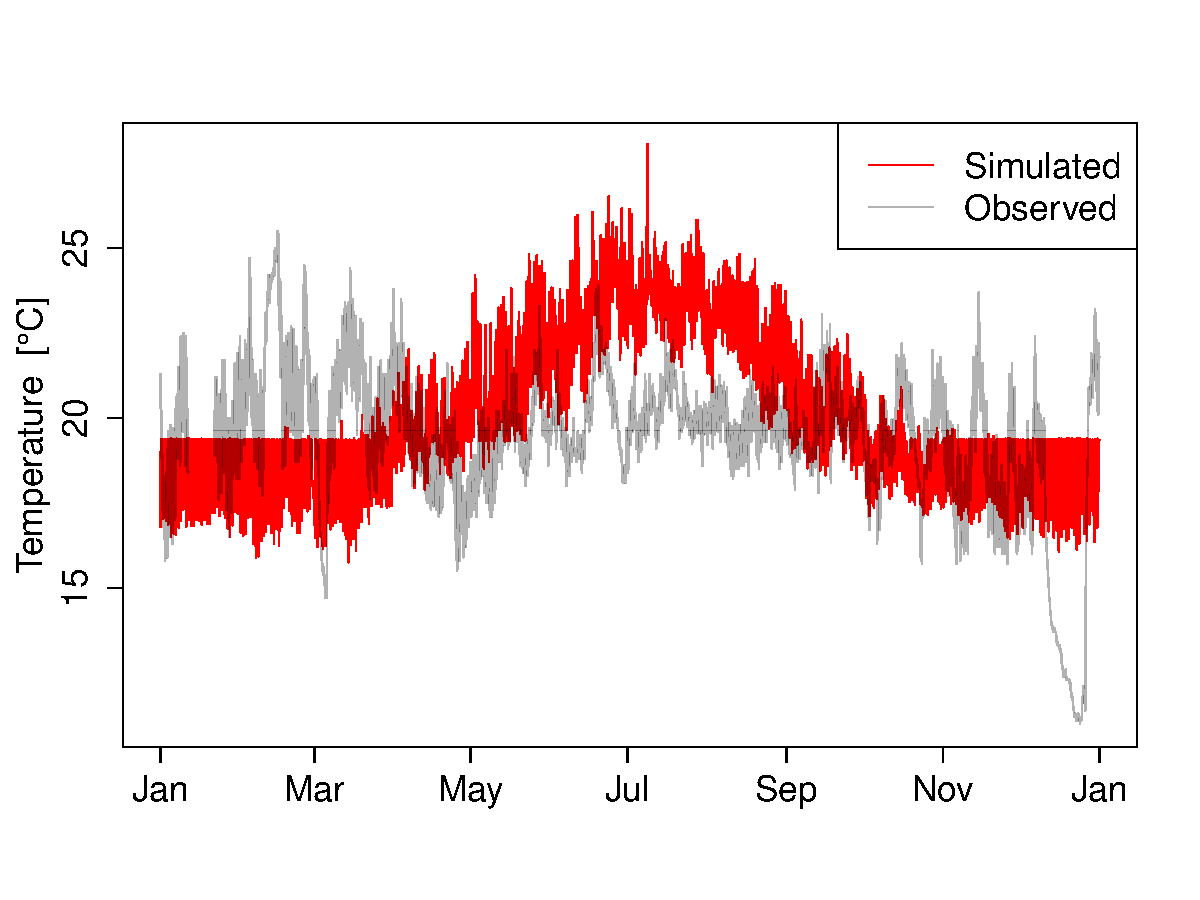
\includegraphics[scale=\scl]{Temperatures/Simulated/Sim_Kitch_949}
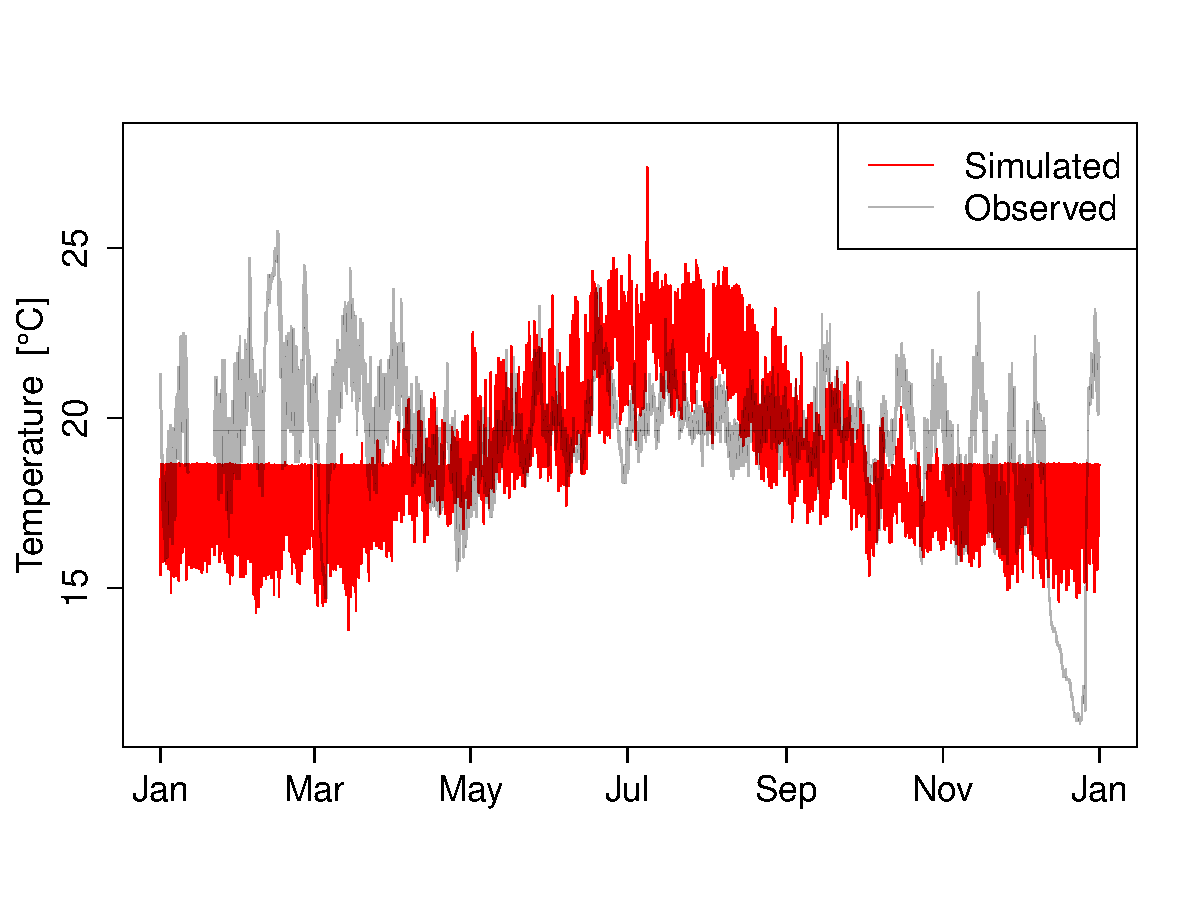
\includegraphics[scale=\scl]{Temperatures/Simulated/Sim_Kitch_71_noylab}\caption{Four examples of simulated kitchen temperature (red). The time series of observed temperature is overlapped in gray. Details of simulated temperature vary from one run to the other, but all plots show major common features: a simulation-dependent threshold temperature is reached daily during colder months, while temperature follows a ``bow'' shape in between.}
\label{Fig_Sim_Temp}
\end{figure}

\autoref{Fig_Sim_Temp} shows examples of simulated kitchen temperature time series. The main feature that those plots reveal is as follows: during colder months, simulated temperature is not allowed to exceed a given threshold, whose value is characteristic to the simulation.
Investigation of the relationship between this value and the eight simulation inputs for the 1000 design runs shows that the threshold temperature value is in fact equal to the heating setpoint value specified for each simulation (variable $V_1$ in \autoref{Table_Var_names}). 
As \autoref{Fig_Zoom} reveals, this threshold is reached periodically and maintained for some time before dropping. Temperature is then quickly restored to the desired value, in a sequence of cycles each lasting a few hours.



\begin{figure}
\centering
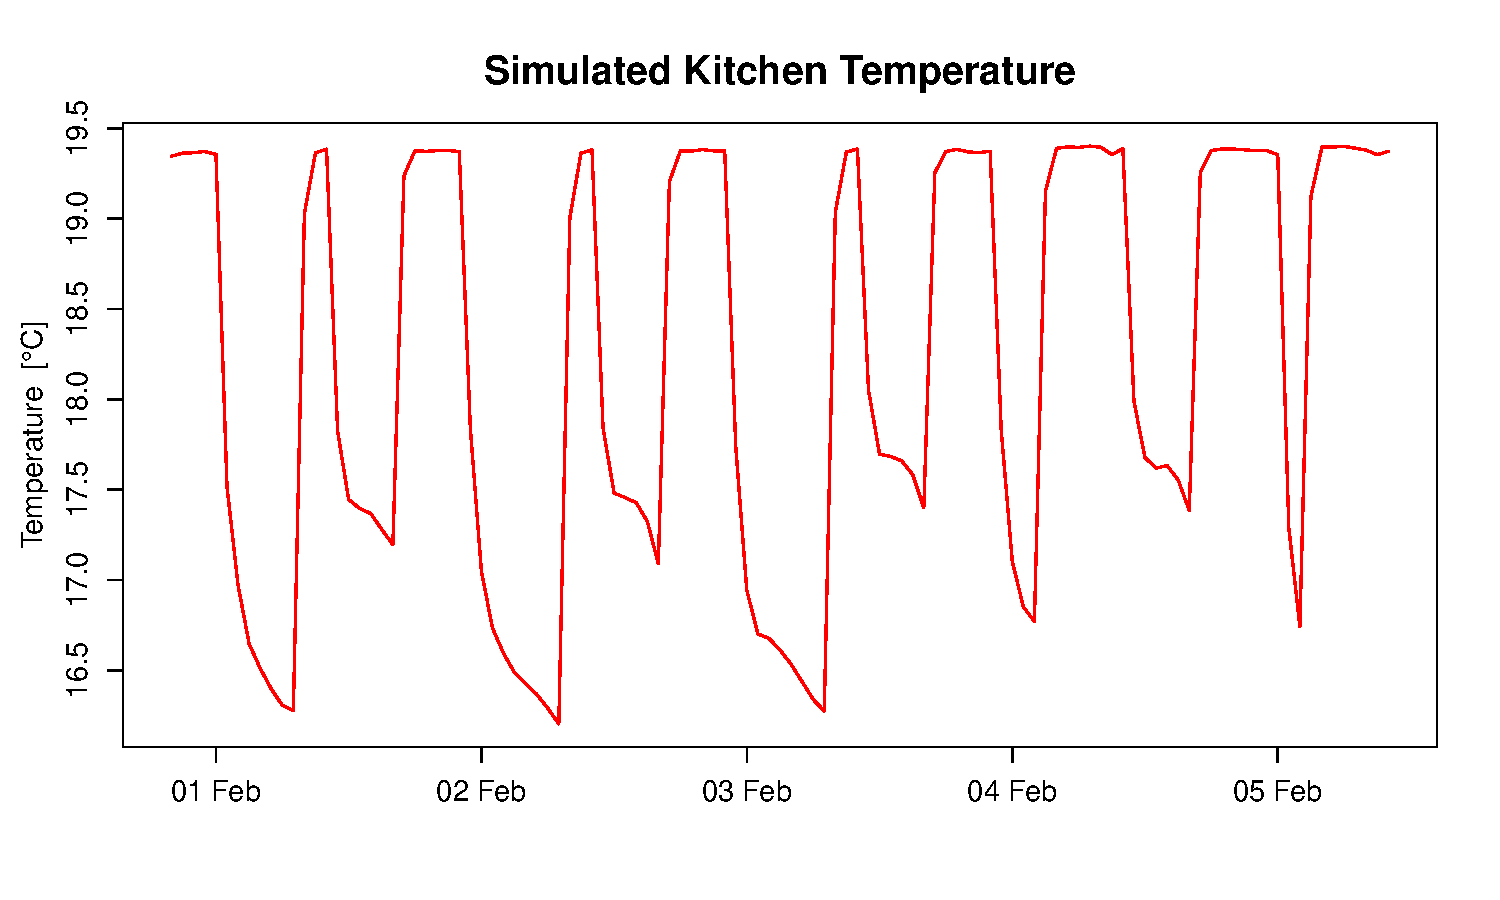
\includegraphics[scale=0.63]{Temperatures/Zoom_570}
\caption{Simulated temperature for one of the design runs during a period of a few days at the beginning of February. The pattern is representative of all simulated temperatures during cold months: a threshold temperature corresponding to the value of the heating set point is reached every few hours, with temperature drops in between any two such periods.  }
\label{Fig_Zoom}
\end{figure}

\textcolor{red}{\bf \underline{Note for Mohammad}}: while analysing the data, I noticed that all simulations have a sudden peak in temperature (of about 3 degrees) during the afternoon of the $8^\text{th}$ of July. That's also visible in all panels of \autoref{Fig_Sim_Temp}. This will likely have no effect on our analyses, but I genuinely wondered what may have been set in the model that has triggered this peculiar behaviour across all simulations.


\subsection{Comparing Observed and Simulated Temperature}

Given two time series of length $N$, one way of summarising the extent to which they differ is to compute the squared $L^2$ difference between the two. In our case, if $S$ is a simulated temperature time series and $M$ is the time series of actual measures, we can consider the following:
\begin{equation}
\D(S,M) = \frac{1}{N} \sum_{i=1}^N {(M_i - S_i)}^2,
\end{equation}
where the index $i$ represents time, $i=1, \dots, N=8760$ in our case.





















\end{document}
